% Template adapted from https://github.com/jgm/pandoc-templates/blob/master/default.latex
% To be used with XeLaTex in memoiR
%%%%%%%%%%%%%%%%%%%%%%%%%%%%%%%%%%%%%%%%%%%%%%%%%%%%%%%%%%%%%%%%%%%%%%%%%%%%%%%%%%%%%%%%%

% Options for packages loaded elsewhere
\PassOptionsToPackage{unicode=true}{hyperref}
\PassOptionsToPackage{hyphens}{url}
\PassOptionsToPackage{dvipsnames,svgnames*,x11names*}{xcolor}
% Right to left support


\documentclass[
  12pt,
  american,
  a4paper,
  extrafontsizes,onecolumn,openright
  ]{memoir}

% Double (or whatever) spacing

% Math
\usepackage{amssymb, amsmath}
% mathspec: arbitrary math fonts
\usepackage{unicode-math}
\defaultfontfeatures{Scale=MatchLowercase}
\defaultfontfeatures[\rmfamily]{Ligatures=TeX,Scale=1}

% Fonts
\usepackage{lmodern}
\usepackage{fontspec}
% Main font
% Specific sanserif font
% Specific monotype font
% Specific math font
% Chinese, Japanese, Corean fonts

% Use upquote for straight quotes in verbatim environments
\usepackage{upquote}
% Use microtype
\usepackage[]{microtype}
\UseMicrotypeSet[protrusion]{basicmath} % disable protrusion for tt fonts

% Verbatim in note

% Color links
\usepackage{xcolor}

% Strikeout

% Necessary for code chunks
\usepackage{color}
\usepackage{fancyvrb}
\newcommand{\VerbBar}{|}
\newcommand{\VERB}{\Verb[commandchars=\\\{\}]}
\DefineVerbatimEnvironment{Highlighting}{Verbatim}{commandchars=\\\{\}}
% Add ',fontsize=\small' for more characters per line
\usepackage{framed}
\definecolor{shadecolor}{RGB}{248,248,248}
\newenvironment{Shaded}{\begin{snugshade}}{\end{snugshade}}
\newcommand{\AlertTok}[1]{\textcolor[rgb]{0.94,0.16,0.16}{#1}}
\newcommand{\AnnotationTok}[1]{\textcolor[rgb]{0.56,0.35,0.01}{\textbf{\textit{#1}}}}
\newcommand{\AttributeTok}[1]{\textcolor[rgb]{0.77,0.63,0.00}{#1}}
\newcommand{\BaseNTok}[1]{\textcolor[rgb]{0.00,0.00,0.81}{#1}}
\newcommand{\BuiltInTok}[1]{#1}
\newcommand{\CharTok}[1]{\textcolor[rgb]{0.31,0.60,0.02}{#1}}
\newcommand{\CommentTok}[1]{\textcolor[rgb]{0.56,0.35,0.01}{\textit{#1}}}
\newcommand{\CommentVarTok}[1]{\textcolor[rgb]{0.56,0.35,0.01}{\textbf{\textit{#1}}}}
\newcommand{\ConstantTok}[1]{\textcolor[rgb]{0.00,0.00,0.00}{#1}}
\newcommand{\ControlFlowTok}[1]{\textcolor[rgb]{0.13,0.29,0.53}{\textbf{#1}}}
\newcommand{\DataTypeTok}[1]{\textcolor[rgb]{0.13,0.29,0.53}{#1}}
\newcommand{\DecValTok}[1]{\textcolor[rgb]{0.00,0.00,0.81}{#1}}
\newcommand{\DocumentationTok}[1]{\textcolor[rgb]{0.56,0.35,0.01}{\textbf{\textit{#1}}}}
\newcommand{\ErrorTok}[1]{\textcolor[rgb]{0.64,0.00,0.00}{\textbf{#1}}}
\newcommand{\ExtensionTok}[1]{#1}
\newcommand{\FloatTok}[1]{\textcolor[rgb]{0.00,0.00,0.81}{#1}}
\newcommand{\FunctionTok}[1]{\textcolor[rgb]{0.00,0.00,0.00}{#1}}
\newcommand{\ImportTok}[1]{#1}
\newcommand{\InformationTok}[1]{\textcolor[rgb]{0.56,0.35,0.01}{\textbf{\textit{#1}}}}
\newcommand{\KeywordTok}[1]{\textcolor[rgb]{0.13,0.29,0.53}{\textbf{#1}}}
\newcommand{\NormalTok}[1]{#1}
\newcommand{\OperatorTok}[1]{\textcolor[rgb]{0.81,0.36,0.00}{\textbf{#1}}}
\newcommand{\OtherTok}[1]{\textcolor[rgb]{0.56,0.35,0.01}{#1}}
\newcommand{\PreprocessorTok}[1]{\textcolor[rgb]{0.56,0.35,0.01}{\textit{#1}}}
\newcommand{\RegionMarkerTok}[1]{#1}
\newcommand{\SpecialCharTok}[1]{\textcolor[rgb]{0.00,0.00,0.00}{#1}}
\newcommand{\SpecialStringTok}[1]{\textcolor[rgb]{0.31,0.60,0.02}{#1}}
\newcommand{\StringTok}[1]{\textcolor[rgb]{0.31,0.60,0.02}{#1}}
\newcommand{\VariableTok}[1]{\textcolor[rgb]{0.00,0.00,0.00}{#1}}
\newcommand{\VerbatimStringTok}[1]{\textcolor[rgb]{0.31,0.60,0.02}{#1}}
\newcommand{\WarningTok}[1]{\textcolor[rgb]{0.56,0.35,0.01}{\textbf{\textit{#1}}}}

% Listings package

% Tables
\usepackage{longtable,booktabs,tabu}
% Fix footnotes in tables (requires footnote package)
\IfFileExists{footnote.sty}{\usepackage{footnote}\makesavenoteenv{longtable}}{}

% Graphics
\usepackage{graphicx,grffile}
\graphicspath{{images/}}
\makeatletter
\def\maxwidth{\ifdim\Gin@nat@width>\linewidth\linewidth\else\Gin@nat@width\fi}
\def\maxheight{\ifdim\Gin@nat@height>\textheight\textheight\else\Gin@nat@height\fi}
\makeatother
% Scale images if necessary, so that they will not overflow the page
% margins by default, and it is still possible to overwrite the defaults
% using explicit options in \includegraphics[width, height, ...]{}
\setkeys{Gin}{width=\maxwidth,height=\maxheight,keepaspectratio}

% Prevent overfull lines
\setlength{\emergencystretch}{3em}  
\providecommand{\tightlist}{%
  \setlength{\itemsep}{0pt}\setlength{\parskip}{0pt}}

% Number sections for memoir (secnumdepth counter is ignored)
\setsecnumdepth{section}

% Set default figure placement to htbp
\makeatletter
\def\fps@figure{htbp}
\makeatother

% Spacing in lists
\usepackage{enumitem}

% Polyglossia
\usepackage{polyglossia}
\setmainlanguage{en-US}
\setotherlanguage{fr-FR}
\setotherlanguage{it}

% BibLaTeX
\usepackage[backend=biber,style=authoryear-ibid,isbn=false,backref=true,giveninits=true,uniquename=init,maxcitenames=2,maxbibnames=150,sorting=nyt,sortcites=false]{biblatex}
\addbibresource{references.bib}

% cslreferences environment required by pandoc > 2.7



%%%%%%%%%%%%%%%%%%%%%%%%%%%%%%%%%%%%%%%%%%%%%%%%%%%%%%%%%%
% memoiR format

% Chapter Summary environment 
\usepackage[tikz]{bclogo}
\newenvironment{Summary}
  {\begin{bclogo}[logo=\bctrombone, noborder=true, couleur=lightgray!50]{In a Nutshell}\parindent0pt}
  {\end{bclogo}}
% Syntax:
%
%```{block, type='Summary'}
% Deliver message here.
% ```

% scriptsize code 
\let\oldverbatim\verbatim
\def\verbatim{\oldverbatim\scriptsize}
% Applies to code blocks and R code results
% code chunk options size='scriptsize' applies only to R code and results
% if the code chunk sets a different size, \def\verbatim{...} is prioritary for code results 


% Layout
%%%%%%%%%%%%%%%%%%%%%%%%%%%%%%%%%%%%%%%%%%%%%%%%%%%%%%%%%%

% Based on memoir, style companion
\newcommand{\MemoirChapStyle}{daleif1}
\newcommand{\MemoirPageStyle}{Ruled}

% Space between paragraphs
\usepackage{parskip}
  \abnormalparskip{3pt}

% Adjust margin paragraphs vertical position
\usepackage{marginfix}


% Margins
%%%%%%%%%%%%%%%%%%%%%%%%%%%%%%%%%%%%%%%

% allow use of '-',+','/' ans '*' to make simple length computation
\usepackage{calc}

% Full-width figures utilities
\newlength\widthw % full width
\newlength{\rf}
\newcommand*{\definesHSpace}{
  \strictpagecheck % slower but efficient detection of odd/even pages
  \checkoddpage
  \ifoddpage
  \setlength{\rf}{0mm}
  \else
  \setlength{\rf}{\marginparsep+\marginparwidth}
  \fi
}

\makeatletter
% 1" margins for the front matter.
\newcommand*{\SmallMargins}{
  \setlrmarginsandblock{1.5in}{1.5in}{*}
  \setmarginnotes{0.1in}{0.1in}{0.1in}
 \setulmarginsandblock{1.5in}{1in}{*}
  \checkandfixthelayout
  \ch@ngetext
  \clearpage
  \setlength{\widthw}{\textwidth+\marginparsep+\marginparwidth}
  \footnotesatfoot
  \chapterstyle{\MemoirChapStyle}  % Chapter and page styles must be recalled
  \pagestyle{\MemoirPageStyle}
}

% 3" outer margin for the main matter
\newcommand{\LargeMargins}{\SmallMargins}
\makeatother

% Figure captions and footnotes in outer margins


% Main title page with filigrane
%%%%%%%%%%%%%%%%%%%%%%%%%%%%%%%%%%%%%%%%%%%%%%%%%%%%%%%%%%

% Text blocks
\usepackage[absolute,overlay]{textpos}
  \setlength{\TPHorizModule}{1mm}
  \setlength{\TPVertModule}{1mm}

\newcommand{\MainTitlePage}[2]{
  \SmallMargins % Margins
  \pagestyle{empty} % No header/footer
  \textblockorigin{\stockwidth-\paperwidth-\trimedge}{\trimtop} % recto
  \begin{textblock*}{2mm}(\spinemargin/2,\uppermargin/2)
    \rule{1pt}{\paperheight-\uppermargin}
  \end{textblock*}
  \begin{textblock*}{\paperwidth*2/3}(\paperwidth/5, \paperheight/5)
    \flushright
    \begin{Spacing}{3}
      {\fontfamily{qtm}\selectfont\fontsize{45}{45}\selectfont\textsc{\thetitle}}
    \end{Spacing}
  \end{textblock*}
    \begin{textblock*}{\paperwidth*2/3}(\paperwidth/5, \paperheight/2)
    \flushright
    {\fontfamily{qtm}\huge\theauthor}
  \end{textblock*}
    \begin{textblock*}{\paperwidth*2/3}[0, 1](\spinemargin, \uppermargin+\textheight)
    \normalfont\thedate
  \end{textblock*}
  ~\\ % Print a character or the page will not exist
  \newpage
  \textblockorigin{\trimedge}{\trimtop} % verso
  \begin{textblock*}{\textwidth}(\paperwidth-\spinemargin-\textwidth, \uppermargin)
    #1
  \end{textblock*}
  \begin{textblock*}{\textwidth}[0,1](\paperwidth-\spinemargin-\textwidth, \uppermargin+\textheight+\footskip)
    \centering
    \includegraphics[width=\paperwidth/4]{logo}\\ \bigskip
    #2
  \end{textblock*}
  ~\\ % Print a character or the page will not exist
  \newpage
}

% Clear page and open an even one (\clearpage opens an odd one)
\newcommand{\evenpage}{
  \clearpage
  \strictpagecheck % slower but efficient detection of odd/even pages
  \checkoddpage
  \ifoddpage
    \thispagestyle{empty}
    ~\\ % Print a character or the page will not exist
    \newpage
  \else
    % do nothing
  \fi
}


%% PDF title page to insert
%%%%%%%%%%%%%%%%%%%%%%%%%%%%%%%%%%%%%%%%%%%%%%%%%%%%%%%%%%



%% Bibliography
%%%%%%%%%%%%%%%%%%%%%%%%%%%%%%%%%%%%%%%%%%%%%%%%%%%%%%%%%%

\usepackage[strict,autostyle]{csquotes}
% Repeated citation as author-year-title instead of author-title (modification of footcite:note in verbose-inote.cbx)

%% Table of Contents
%%%%%%%%%%%%%%%%%%%%%%%%%%%%%%%%%%%%%%%%%%%%%%%%%%%%%%%%%%

% fix the typesetting of the part number
\renewcommand\partnumberlinebox[2]{#2\ ---\ }


% Fonts
%%%%%%%%%%%%%%%%%%%%%%%%%%%%%%%%%%%%%%%%%%%%%%%%%%%%%%%%%%


% Hyperref comes last
%%%%%%%%%%%%%%%%%%%%%%%%%%%%%%%%%%%%%%%%%%%%%%%%%%%%%%%%%%

\usepackage{hyperref}
\hypersetup{
  pdftitle={Modélisation de la régénération d'espèces semi-héliophiles de Guyane sur un gradient de perturbations naturelles et anthropiques},
  pdfauthor={Marine Boudy},
  colorlinks=true,
  linkcolor=Maroon,
  citecolor=Blue,
  urlcolor=Blue,
  breaklinks=true}

% Don't use monospace font for urls
\urlstyle{same}


% Title, author, date from YAML to LaTeX
%%%%%%%%%%%%%%%%%%%%%%%%%%%%%%%%%%%%%%%%%%%%%%%%%%%%%%%%%%

\title{Modélisation de la régénération d'espèces semi-héliophiles de Guyane sur un gradient de perturbations naturelles et anthropiques}

\author{Marine Boudy}

\date{2022-04-28}


% Include headers (preamble.tex) here
%%%%%%%%%%%%%%%%%%%%%%%%%%%%%%%%%%%%%%%%%%%%%%%%%%%%%%%%%%
% Add LaTeX code into the preamble of the document here
\hyphenation{bio-di-ver-si-ty sap-lings}


%%%%%%%%%%%%%%%%%%%%%%%%%%%%%%%%%%%%%%%%%%%%%%%%%%%%%%%%%%%%%%%%%%%%%%%%%
% memoiR dalef3 chapter style 
% https://ctan.crest.fr/tex-archive/info/latex-samples/MemoirChapStyles/MemoirChapStyles.pdf
\usepackage{soul}
\definecolor{nicered}{rgb}{.647,.129,.149}
\makeatletter
\newlength\dlf@normtxtw
\setlength\dlf@normtxtw{\textwidth}
\def\myhelvetfont{\def\sfdefault{mdput}}
\newsavebox{\feline@chapter}
\newcommand\feline@chapter@marker[1][4cm]{%
  \sbox\feline@chapter{%
    \resizebox{!}{#1}{\fboxsep=1pt%
	  \colorbox{nicered}{\color{white}\bfseries\sffamily\thechapter}%
	}}%
  \rotatebox{90}{%
    \resizebox{%
	  \heightof{\usebox{\feline@chapter}}+\depthof{\usebox{\feline@chapter}}}%
	{!}{\scshape\so\@chapapp}}\quad%
  \raisebox{\depthof{\usebox{\feline@chapter}}}{\usebox{\feline@chapter}}%
 }
\newcommand\feline@chm[1][4cm]{%
  \sbox\feline@chapter{\feline@chapter@marker[#1]}%
  \makebox[0pt][l]{% aka \rlap
    \makebox[1cm][r]{\usebox\feline@chapter}%
  }}
\makechapterstyle{daleif1}{
  \renewcommand\chapnamefont{\normalfont\Large\scshape\raggedleft\so}
  \renewcommand\chaptitlefont{\normalfont\huge\bfseries\scshape\color{nicered}}
  \renewcommand\chapternamenum{}
  \renewcommand\printchaptername{}
  \renewcommand\printchapternum{\null\hfill\feline@chm[2.5cm]\par}
  \renewcommand\afterchapternum{\par\vskip\midchapskip}
  \renewcommand\printchaptertitle[1]{\chaptitlefont\raggedleft ##1\par}
}
\makeatother
\usepackage{booktabs}
\usepackage{longtable}
\usepackage{array}
\usepackage{multirow}
\usepackage{wrapfig}
\usepackage{float}
\usepackage{colortbl}
\usepackage{pdflscape}
\usepackage{tabu}
\usepackage{threeparttable}
\usepackage{threeparttablex}
\usepackage[normalem]{ulem}
\usepackage{makecell}
\usepackage{xcolor}


% End of preamble
%%%%%%%%%%%%%%%%%%%%%%%%%%%%%%%%%%%%%%%%%%%%%%%%%%%%%%%%%%


\begin{document}
\frontmatter

% Title page
%%%%%%%%%%%%%%%%%%%%%%%%%%%%%%%%%%%%%%%%%%%%%%%%%%%%%%%%%%


\MainTitlePage{This document is reproducible thanks to:

\begin{itemize}
  \item \LaTeX and its class memoir (\url{http://www.ctan.org/pkg/memoir}).
  \item R (\url{http://www.r-project.org/}) and RStudio (\url{http://www.rstudio.com/})
  \item bookdown (\url{http://bookdown.org/}) and memoiR (\url{https://ericmarcon.github.io/memoiR/})
\end{itemize}}{Name of the owner of the logo

\url{http://www.company.com}

An explanatory sentence.
Leave an empty line for line breaks.}


% Before Body
%%%%%%%%%%%%%%%%%%%%%%%%%%%%%%%%%%%%%%%%%%%%%%%%%%%%%%%%%%





% Contents
%%%%%%%%%%%%%%%%%%%%%%%%%%%%%%%%%%%%%%%%%%%%%%%%%%%%%%%%%%

\LargeMargins
{
\hypersetup{linkcolor=}
\setcounter{tocdepth}{2}
\tableofcontents
}


% Body
%%%%%%%%%%%%%%%%%%%%%%%%%%%%%%%%%%%%%%%%%%%%%%%%%%%%%%%%%%

\LargeMargins
\hypertarget{introduction}{%
\chapter*{Introduction}\label{introduction}}
\addcontentsline{toc}{chapter}{Introduction}

Ce gitbook est un document de travail provisoire, qui servira de support pour le suivi du stage de fin d'étude et la rédaction du mémoire de fin d'études de Marine Boudy.

\mainmatter

\hypertarget{point-duxe9tape-3e-semaine-de-stage}{%
\chapter{\texorpdfstring{Point d'étape: 3\textsuperscript{e} semaine de stage}{Point d'étape: 3e semaine de stage}}\label{point-duxe9tape-3e-semaine-de-stage}}

\hypertarget{probluxe9matique-du-stage}{%
\section{Problématique du stage}\label{probluxe9matique-du-stage}}

En Guyane française, les espèces exploitées ont majoritairement un comportement semi-héliophile, c'est à dire que les jeunes stades de développement ont besoin de lumière pour croître mais peuvent entrer en stade d'attente en l'absence de celle ci. De plus, l'exploitation forestière en forêt tropicale a principalement lieu en des forêts peu perturbées. Afin de garantir la durabilité de la ressource en bois il est donc nécessaire que les méthodes d'exploitation forestières permettent la régénération des espèces exploitées, pour garantir le potentiel de reproduction de ces dernières. Dans le cas des forêts guyanaises, cela passe par le maintien d'une dynamique de peuplement le plus proche possible de la dynamique naturelle \autocite{Guitet2014}. La norme pour les aménagements forestiers est aujourd'hui l'Exploitation Faible Impact (EFI) depuis 2010 \autocite{ONF2017}. Cette méthode doit garantir « une opération d'exploitation forestière intensément planifiée, précautionneusement mise en œuvre et contrôlée afin de minimiser son impact sur le peuplement et les sols forestiers, et se basant habituellement sur une sélection des individus à abattre» (FAO,2004 in \autocite{ONF2017}). Les préconisations liées à l'exploitation sont ainsi réunies dans la Charte EFI: désignation, exploitation d'une faible densité de tige à l'hectare, rotations de 65 ans\ldots{}

La modélisation de la structure et de la dynamique des peuplements peut contribuer à évaluer les impacts de l'exploitation et des autres perturbations d'origine anthropique ou climatique sur les peuplements forestiers \autocite{Fargeon2016},\autocite{Fischer2016},\autocite{Gourlet-Fleury2005a}. Or, un des manques de ces modèles concerne les stades de développement des arbres de diamètre inférieurs à 10 cm \autocite{Gourlet-Fleury2005a}. En effet, peu de données exploitables sont disponibles sur la croissance et les affinités environnementales de ces stades ontogéniques, et la majorité des modèles de croissance ne permettent l'analyse des dynamiques de peuplement qu'à partir des classes de diamètre supérieures à 10cm \autocite{Herault2010d}.

La lumière disponible est un des principaux facteurs abiotiques influençant la présence de plantules et le développement de juvéniles établis. Or, en forêt tropicale humide, la mise en lumière de la régénération se fait principalement à proximité de zone de trouées ou « chablis ». L'ouverture de trouées provient d'une part de phénomènes naturels tels que la chute d'arbres brisés ou déracinés, la chute de grosses branches ; l'exploitation forestière génère également des trouées à l'emplacement des arbres exploités, des pistes et des places de retournement ou de dépôt. La réponse de la régénération au gradient de lumière généré par les trouées a fait l'objet de nombreuses études \autocite{Poorter1999}, \autocite{Sheil2006} ,\autocite{Ruger2011a},\autocite{Laurans2012},\autocite{Zhu2014}.

Pourtant, peu d'études ont inclut le facteur lumière dans la modélisation de la démographie des espèces, car ce facteur présente de fortes variabilités temporelles et spatiales (Ferment et al, 2001),(Hérault,2010). Aujourd'hui, l'accès à des données LiDAR permet l'obtention de mesures précises et objectives des trouées dans la canopée et constitue une réelle opportunité pour la compréhension de la démographie des espèces dépendantes à la lumière, dont les espèces semi-héliophiles \autocite{Hunter2015},\autocite{Goulamoussene2017},\autocite{Rangel2019},\autocite{Stark2015}.

La thèse intitulée « Effet de la dynamique de canopée de forêt exploitée sur les populations d'espèces d'arbres récoltées en Guyane », en appui duquel a lieu ce stage, va aborder la question de la modélisation de la croissance des individus de diamètre supérieur à 10 cm pour 11 espèces considérées comme semi-héliophiles, dont 7 appartiennent aux Essences Commerciales Majeures Principales(ECMP) en intégrant le facteur lumière.
La problématique du stage est donc la suivante: Comment modéliser le recrutement des espèces semi-héliophiles étudiées en prenant en compte le facteur lumière?
Les modèles de recrutement obtenus seront dans une étape ultérieure intégrés à un simulateur de dynamique du peuplement. Les individus étudiés ici sont regroupés sous le terme de ``juvéniles'', et correspondent aux tiges de plus de 30cm de haut et au diamètre inférieur à 10cm.

Ainsi, ce stage a pour objectif de répondre aux questions suivantes :

\begin{enumerate}
\def\labelenumi{\arabic{enumi})}
\tightlist
\item
  Quelles variables retenir pour caractériser la présence de la régénération d'espèces ligneuses exploitées au stade juvénile?
  La lumière étant un facteur environnemental important pour la croissance des individus, quelles sont les conditions de lumière qui déterminent l'établissement de la régénération de l'espèce étudiées ?
  En particulier, qu'en est-il pour les espèces dont les juvéniles ont un caractère semi-héliophiles ?
\end{enumerate}

Pour chacune des espèces semi-héliophiles étudiées, il s'agit d'une part d'identifier les variables à expliquer, ainsi que les variables explicatives.

Parmi les variables à expliquer, plusieurs ont déjà étés étudiées avec des résultats variables selon l'espèce et le site d'étude :

\begin{itemize}
\item
  Nombre d'individus par espèce.
\item
  Densité d'individus par espèce à l'hectare.
\item
  Hauteur moyenne, médiane et cumulée des individus.
\end{itemize}

Plusieurs variables explicatives de l'influence de la lumière sont envisagées :

\begin{itemize}
\item
  Distance de la placette à la trouée.
\item
  Surface de la trouée la plus proche.
\item
  Proportion de la surface de la placette impactée par la trouee (création de zones tampon de 5, 10 ou 15 m autour de la trouee et analyse de la surface de recouvrement entre les zones tampon et la placette).
\item
  Intersection d'une zone tampon autour de la placette avec les trouées (création de zones tampon de 5, 10 ou 15 m autour de la placette et analyse de la surface de recouvrement entre les zones tampon et la trouee).
\item
  Hauteur moyenne, dominante, quartiles de la hauteur des arbres de la canopée entourant la trouée, mesurés dans des zones tampon autour de la trouée.
\end{itemize}

Des variables explicatives autres que des proxy de la lumière sont envisagées

\begin{itemize}
\item
  Un des indice les plus utilisé pour mesurer le stade ontogénique d'un individu est le rapport DBH/DBH95. Or, il est connu que les juvéniles ont une plus forte croissance en hauteur qu'en diamètre; il serait donc intéressant de créer un indice Hauteur/Hauteur maximum (La hauteur maximum(Hmax) correspondant à la hauteur Maximum de l'espèce obtenu a partir d'un équation d'allométiee prenant en compte le DBH 95.
\item
  La compétition vis-à-vis des espèces ligneuses présentes dans la régénération, autres que celles étudiées.
\item
  Le Topographic Wetness Index (TWI) pour quantifier l'effet de la topographie.
\end{itemize}

Des modèles Zero-inflated Poisson seront construits à partir des variables les plus pertinentes pour chaque espèce.

\begin{enumerate}
\def\labelenumi{\arabic{enumi})}
\setcounter{enumi}{1}
\tightlist
\item
  Comment intégrer les informations obtenues aux étapes précédentes dans un modèle de recrutement ?
\end{enumerate}

Il s'agira de construire le modèle de recrutement le plus adapté pour chaque espèce. Pour cela, nous évaluerons entre autres comment simuler les variables explicatives retenues et fixer le nombre d'arbres recrutés en cohérence avec les données démographiques connues des arbres de diamètre supérieur à 10 cm.

\hypertarget{duxe9rouluxe9-du-stage}{%
\section{Déroulé du stage}\label{duxe9rouluxe9-du-stage}}

Afin de répondre aux questions précédentes, le stage est divisé en une phase d'inventaire de terrain et une phase d'analyse et de modélisation. Le planning du stage est décrit sur la figure suivante.

\scriptsize

\begin{figure}

{\centering 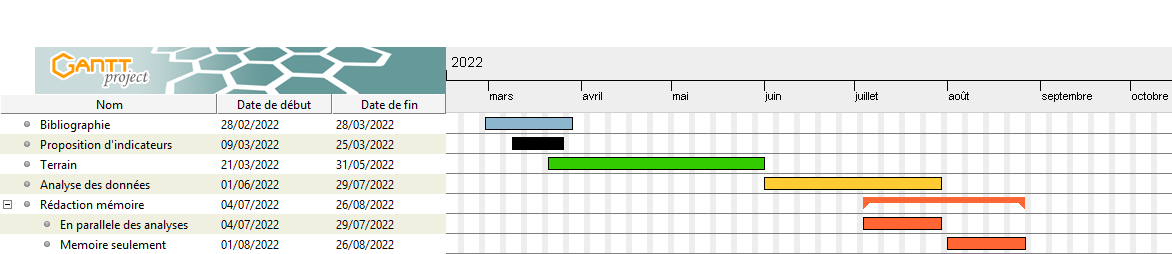
\includegraphics[width=1\linewidth]{images/chronogramme} 

}

\caption{Chronogramme du stage}\label{fig:planning}
\end{figure}

\normalsize

Le terrain se fera dans les forêts de Paracou et Régina Saint-Georges, pour lesquelles sont disponibles des données d'inventaires des arbres adultes, ainsi que des données issues du LiDAR à partir desquelles une pré-identification des zones de trouées est faite.

\textbf{Protocole d'échantillonnage :}

Les trouées de plus de 10 m\textsuperscript{2} sont préalablement repérées via le Modèle Numérique de Canopée (MNC) issu des données LiDAR. Ces trouées sont donc géoréférencées. Lors de la phase terrain, chacune de ces trouées est parcourue. Un inventaire est réalisé dans les cas où un semencier d'une des espèces cibles est présent à proximité de la trouées, et si des individus juvéniles de notre liste d'espèce sont présents à proximité de la trouée.

\textbf{Effort d'échantillonnage:}

En moyenne, 12 placettes d'inventaire sont réalisable pour deux opérateur en une journée de terrain.

12 semaines soit 60 jours de terrain sont prévus, une marge de quelques jours étant nécessaire du fait des conditions météorologiques. Ainsi, 720 placettes pourront, au maximum, être réalisées dans le cadre de ce stage. En plus de cet inventaire, seront intégrées à l'analyse les données de 2 stages de 2 mois réalisés en 2021 \autocite{Pierre-Justin2021} et 2022 \autocite{Van2022} selon le même protocole .

\textbf{Protocole d'inventaire :}
Les espèces inventoriées sont les suivantes: \emph{Dicorynia guianensis}, \emph{Qualea rosa}, \emph{Eperua falcata}, \emph{Eperua grandiflora}, \emph{Qualea albiflora}, \emph{Peltogyne spp}, \emph{Manilkara bidentata}, \emph{Manilkara huberii}, \emph{Sextonia rubra}, \emph{Goupia glabra}, \emph{Bagassa guianensis}, \emph{Vouacapoua americana}.

Au niveau des trouées d'intérêt repérées via les données lidar et des données d'exploitation géoréférencées, 4 placettes de 5m de rayon sont inventorié par trouées :

\begin{itemize}
\item
  Une placette est placée à proximité de la souche de l'arbre tombé.
\item
  Une 2\textsuperscript{e} à proximité du houppier de l'arbre.
\item
  Une 3\textsuperscript{e} en lisière du chablis, lorsque la trouée est suffisamment grande.
\item
  Une 4\textsuperscript{e} à distance du chablis, en se plaçant si possible sous couvert forestier.
\end{itemize}

Dans chaque placette sont inventoriés les individus des 11 espèces présentant une hauteur supérieure à 30 cm et un diamètre inférieur à 10 cm:

\begin{itemize}
\item
  La hauteur de chaque individu est mesurée à l'aide d'un télémètre ou d'un mètre.
\item
  Le diamètre des tiges de plus de 1,3 m de haut est mesuré au pied à coulisse.
\end{itemize}

La hauteur des 3 plus hautes tiges ne faisant pas partie de la liste d'espèces à inventorier est également mesurée. Cette mesure permet d'avoir une idée de la compétition entre nos espèces d'intérêt et les autres.

\#Creation de variables

\scriptsize

\begin{Shaded}
\begin{Highlighting}[]
\FunctionTok{library}\NormalTok{(tidyverse)}
\FunctionTok{library}\NormalTok{(readxl)}
\FunctionTok{library}\NormalTok{(sf)}
\FunctionTok{library}\NormalTok{(raster)  }\CommentTok{\# moins rapide que terra qui reprend toutes les fonctions de raster}
\FunctionTok{library}\NormalTok{(rgdal)}
\FunctionTok{library}\NormalTok{(terra)}
\FunctionTok{library}\NormalTok{(rmapshaper)  }\CommentTok{\#pour la conversion polygone vers ligne}
\end{Highlighting}
\end{Shaded}

\normalsize

\scriptsize

\begin{Shaded}
\begin{Highlighting}[]
\CommentTok{\#{-}{-}{-}NUMERIC}
\DocumentationTok{\#\#{-}{-}{-} convertir une colonne en numeric}
\NormalTok{convert\_col\_to\_num }\OtherTok{\textless{}{-}} \ControlFlowTok{function}\NormalTok{(df, my\_col\_name) \{}
\NormalTok{    my\_col }\OtherTok{\textless{}{-}} \FunctionTok{as.numeric}\NormalTok{(df[, my\_col\_name])}
\NormalTok{    df[, my\_col\_name] }\OtherTok{\textless{}{-}}\NormalTok{ my\_col}
    \FunctionTok{return}\NormalTok{(df)}
\NormalTok{\}}
\DocumentationTok{\#\#{-}{-}{-}conversion de plusieurs colones en numeric}
\NormalTok{convert\_multiple\_col\_to\_num }\OtherTok{\textless{}{-}} \ControlFlowTok{function}\NormalTok{(df, my\_col\_names) \{}
\NormalTok{    length\_list }\OtherTok{\textless{}{-}} \FunctionTok{length}\NormalTok{(my\_col\_names)}
    \ControlFlowTok{for}\NormalTok{ (i }\ControlFlowTok{in} \DecValTok{1}\SpecialCharTok{:}\NormalTok{length\_list) \{}
\NormalTok{        df }\OtherTok{\textless{}{-}} \FunctionTok{convert\_col\_to\_num}\NormalTok{(df, my\_col\_names[i])}
\NormalTok{    \}}
    \FunctionTok{return}\NormalTok{(df)}
\NormalTok{\}}
\CommentTok{\#{-}{-}{-}FACTOR}
\DocumentationTok{\#\#{-}{-}{-} convertir une colonne en facteur}
\NormalTok{convert\_col\_to\_factor }\OtherTok{\textless{}{-}} \ControlFlowTok{function}\NormalTok{(df, my\_col\_name) \{}
\NormalTok{    my\_col }\OtherTok{\textless{}{-}} \FunctionTok{as.factor}\NormalTok{(df[, my\_col\_name])}
\NormalTok{    df[, my\_col\_name] }\OtherTok{\textless{}{-}}\NormalTok{ my\_col}
    \FunctionTok{return}\NormalTok{(df)}
\NormalTok{\}}
\DocumentationTok{\#\#{-}{-}{-}conversion de plusieurs colones en facteur}
\NormalTok{convert\_multiple\_col\_to\_factor }\OtherTok{\textless{}{-}} \ControlFlowTok{function}\NormalTok{(df, my\_col\_names) \{}
\NormalTok{    length\_list }\OtherTok{\textless{}{-}} \FunctionTok{length}\NormalTok{(my\_col\_names)}
    \ControlFlowTok{for}\NormalTok{ (i }\ControlFlowTok{in} \DecValTok{1}\SpecialCharTok{:}\NormalTok{length\_list) \{}
\NormalTok{        df }\OtherTok{\textless{}{-}} \FunctionTok{convert\_col\_to\_factor}\NormalTok{(df, my\_col\_names[i])}
\NormalTok{    \}}
    \FunctionTok{return}\NormalTok{(df)}
\NormalTok{\}}
\end{Highlighting}
\end{Shaded}

\normalsize

\scriptsize

\begin{Shaded}
\begin{Highlighting}[]
\DocumentationTok{\#\#\# Import des donnees\#\#\#}
\CommentTok{\#{-}{-}{-}Placette d\textquotesingle{}inventaire}
\NormalTok{plac\_col\_to\_num }\OtherTok{\textless{}{-}} \FunctionTok{c}\NormalTok{(}\StringTok{"XUTM"}\NormalTok{, }\StringTok{"YUTM"}\NormalTok{, }\StringTok{"h1"}\NormalTok{, }\StringTok{"h2"}\NormalTok{, }\StringTok{"h3"}\NormalTok{)}
\NormalTok{placettes }\OtherTok{\textless{}{-}} \FunctionTok{read.csv2}\NormalTok{(}\StringTok{"vault/data/tableur/Placettes\_S9.csv"}\NormalTok{,}
    \AttributeTok{header =} \ConstantTok{TRUE}\NormalTok{, }\AttributeTok{sep =} \StringTok{";"}\NormalTok{, }\AttributeTok{dec =} \StringTok{","}\NormalTok{, }\AttributeTok{fill =} \ConstantTok{TRUE}\NormalTok{) }\SpecialCharTok{\%\textgreater{}\%}
    \FunctionTok{convert\_multiple\_col\_to\_num}\NormalTok{(plac\_col\_to\_num)}
\CommentTok{\#{-}{-}{-}Inventaire des juveniles}
\NormalTok{liste\_col\_to\_num }\OtherTok{\textless{}{-}} \FunctionTok{c}\NormalTok{(}\StringTok{"azimut"}\NormalTok{, }\StringTok{"Distance.au.centre"}\NormalTok{)}
\NormalTok{liste\_col\_to\_factor }\OtherTok{\textless{}{-}} \FunctionTok{c}\NormalTok{(}\StringTok{"Foret"}\NormalTok{, }\StringTok{"Parcelle"}\NormalTok{, }\StringTok{"Carre"}\NormalTok{, }\StringTok{"Essence"}\NormalTok{,}
    \StringTok{"Genre"}\NormalTok{, }\StringTok{"Espece"}\NormalTok{, }\StringTok{"Nom.Vernaculaire"}\NormalTok{, }\StringTok{"Type.placette"}\NormalTok{, }\StringTok{"Traitement"}\NormalTok{)}
\NormalTok{juveniles }\OtherTok{\textless{}{-}} \FunctionTok{read\_excel}\NormalTok{(}\StringTok{"vault/data/tableur/DB\_JUVENILES\_S9\_xl.xlsx"}\NormalTok{,}
    \AttributeTok{sheet =} \StringTok{"DB\_JUVENILES\_S9"}\NormalTok{, }\AttributeTok{col\_names =} \ConstantTok{TRUE}\NormalTok{, }\AttributeTok{guess\_max =} \DecValTok{2000}\NormalTok{) }\SpecialCharTok{\%\textgreater{}\%}
    \FunctionTok{as.data.frame}\NormalTok{() }\SpecialCharTok{\%\textgreater{}\%}
    \FunctionTok{convert\_multiple\_col\_to\_num}\NormalTok{(liste\_col\_to\_num) }\SpecialCharTok{\%\textgreater{}\%}
    \FunctionTok{convert\_multiple\_col\_to\_factor}\NormalTok{(liste\_col\_to\_factor)}
\FunctionTok{save}\NormalTok{(juveniles, }\AttributeTok{file =} \StringTok{"vault/data/juveniles.RData"}\NormalTok{)}
\DocumentationTok{\#\#\# trouees}
\DocumentationTok{\#\#\# arbres parents}
\DocumentationTok{\#\#\# lineaires}
\DocumentationTok{\#\#\#}
\end{Highlighting}
\end{Shaded}

\normalsize

\scriptsize

\begin{Shaded}
\begin{Highlighting}[]
\CommentTok{\#{-}{-}{-}Fonction qui calcule les variables de hauteur pour une essence donnee}
\NormalTok{var\_hauteur\_tot }\OtherTok{\textless{}{-}} \ControlFlowTok{function}\NormalTok{(tableau, code\_essence) \{}
\NormalTok{    juveniles\_hauteur }\OtherTok{\textless{}{-}}\NormalTok{ tableau }\SpecialCharTok{\%\textgreater{}\%}
        \FunctionTok{filter}\NormalTok{(Essence }\SpecialCharTok{==}\NormalTok{ code\_essence) }\SpecialCharTok{\%\textgreater{}\%}
        \FunctionTok{group\_by}\NormalTok{(Nom\_Placette) }\SpecialCharTok{\%\textgreater{}\%}
        \FunctionTok{summarise}\NormalTok{(}\AttributeTok{sumhauteur =} \FunctionTok{sum}\NormalTok{(Hauteur..cm.), }\AttributeTok{hauteur\_moy =} \FunctionTok{mean}\NormalTok{(Hauteur..cm.),}
            \AttributeTok{hauteur\_max =} \FunctionTok{max}\NormalTok{(Hauteur..cm.), }\AttributeTok{hauteur\_min =} \FunctionTok{min}\NormalTok{(Hauteur..cm.)) }\SpecialCharTok{\%\textgreater{}\%}
\NormalTok{        dplyr}\SpecialCharTok{::}\FunctionTok{select}\NormalTok{(Nom\_Placette, sumhauteur, hauteur\_moy,}
\NormalTok{            hauteur\_max, hauteur\_min)}
    \FunctionTok{return}\NormalTok{(juveniles\_hauteur)}
\NormalTok{\}}
\CommentTok{\#{-}{-}{-}Fonction qui calcule les variables de hauteur des individus de moins de 130 cm de hauteur pour une essence donnee}
\NormalTok{var\_inf130 }\OtherTok{\textless{}{-}} \ControlFlowTok{function}\NormalTok{(tableau, code\_essence) \{}
\NormalTok{    juveniles\_inf\_130 }\OtherTok{\textless{}{-}} \FunctionTok{filter}\NormalTok{(juveniles, Essence }\SpecialCharTok{==}\NormalTok{ code\_essence,}
\NormalTok{        Hauteur..cm. }\SpecialCharTok{\textless{}} \DecValTok{130}\NormalTok{) }\SpecialCharTok{\%\textgreater{}\%}
        \FunctionTok{group\_by}\NormalTok{(Nom\_Placette) }\SpecialCharTok{\%\textgreater{}\%}
        \FunctionTok{summarise}\NormalTok{(}\AttributeTok{n\_inf\_130 =} \FunctionTok{n}\NormalTok{(), }\AttributeTok{sum\_h\_inf\_130 =} \FunctionTok{sum}\NormalTok{(Hauteur..cm.),}
            \AttributeTok{mean\_h\_inf\_130 =} \FunctionTok{mean}\NormalTok{(Hauteur..cm.)) }\SpecialCharTok{\%\textgreater{}\%}
\NormalTok{        dplyr}\SpecialCharTok{::}\FunctionTok{select}\NormalTok{(Nom\_Placette, n\_inf\_130, sum\_h\_inf\_130)}
    \FunctionTok{return}\NormalTok{(juveniles\_inf\_130)}
\NormalTok{\}}
\CommentTok{\#{-}{-}{-}Fonction qui calcule les variables de hauteur des individus \textgreater{}= 130 cm de hauteur pour une essence donnee}
\NormalTok{var\_sup130 }\OtherTok{\textless{}{-}} \ControlFlowTok{function}\NormalTok{(tableau, code\_essence) \{}
\NormalTok{    juveniles\_sup\_130 }\OtherTok{\textless{}{-}} \FunctionTok{filter}\NormalTok{(juveniles, Essence }\SpecialCharTok{==}\NormalTok{ code\_essence,}
\NormalTok{        Hauteur..cm. }\SpecialCharTok{\textgreater{}=} \DecValTok{130}\NormalTok{) }\SpecialCharTok{\%\textgreater{}\%}
        \FunctionTok{group\_by}\NormalTok{(Nom\_Placette) }\SpecialCharTok{\%\textgreater{}\%}
        \FunctionTok{summarise}\NormalTok{(}\AttributeTok{n\_sup\_130 =} \FunctionTok{n}\NormalTok{(), }\AttributeTok{sum\_h\_sup\_130 =} \FunctionTok{sum}\NormalTok{(Hauteur..cm.),}
            \AttributeTok{moy\_h\_sup\_130 =} \FunctionTok{mean}\NormalTok{(Hauteur..cm.), }\AttributeTok{diam\_moy =} \FunctionTok{mean}\NormalTok{(Diametre..cm.)) }\SpecialCharTok{\%\textgreater{}\%}
\NormalTok{        dplyr}\SpecialCharTok{::}\FunctionTok{select}\NormalTok{(Nom\_Placette, n\_sup\_130, sum\_h\_sup\_130,}
\NormalTok{            moy\_h\_sup\_130, diam\_moy)}
    \FunctionTok{return}\NormalTok{(juveniles\_sup\_130)}
\NormalTok{\}}
\CommentTok{\#{-}{-}{-}Fonction qui regroupe toutes les données d\textquotesingle{}une essence en un seul tableau tableau}
\NormalTok{tableau\_essence }\OtherTok{\textless{}{-}} \ControlFlowTok{function}\NormalTok{(juveniles, juveniles\_plac, code\_essence) \{}
\NormalTok{    essence\_hauteurs\_tot }\OtherTok{\textless{}{-}} \FunctionTok{var\_hauteur\_tot}\NormalTok{(juveniles, code\_essence)}
\NormalTok{    essence\_sup130 }\OtherTok{\textless{}{-}} \FunctionTok{var\_sup130}\NormalTok{(juveniles, code\_essence)}
\NormalTok{    essence\_infsup130 }\OtherTok{\textless{}{-}} \FunctionTok{var\_inf130}\NormalTok{(juveniles, code\_essence)}
\NormalTok{    juveniles\_essence }\OtherTok{\textless{}{-}}\NormalTok{ juveniles\_plac }\SpecialCharTok{\%\textgreater{}\%}
        \FunctionTok{left\_join}\NormalTok{(essence\_hauteurs\_tot) }\SpecialCharTok{\%\textgreater{}\%}
        \FunctionTok{left\_join}\NormalTok{(essence\_sup130) }\SpecialCharTok{\%\textgreater{}\%}
        \FunctionTok{left\_join}\NormalTok{(essence\_infsup130) }\SpecialCharTok{\%\textgreater{}\%}
        \FunctionTok{as.data.frame}\NormalTok{()}
    \CommentTok{\#{-}{-}{-}Remplace les NA par des 0 pour les variables mesurees sur le terrain}
    \ControlFlowTok{for}\NormalTok{ (i }\ControlFlowTok{in} \FunctionTok{c}\NormalTok{(}\DecValTok{9}\SpecialCharTok{:}\DecValTok{21}\NormalTok{, }\DecValTok{26}\NormalTok{, }\DecValTok{30}\NormalTok{)) \{}
        \CommentTok{\# faire une fonction pour que ce soit moins moche ?}
\NormalTok{        juveniles\_essence[, i][}\FunctionTok{is.na}\NormalTok{(juveniles\_essence[, i])] }\OtherTok{\textless{}{-}} \DecValTok{0}
\NormalTok{    \}}
    \FunctionTok{return}\NormalTok{(juveniles\_essence)}
\NormalTok{\}}
\DocumentationTok{\#\# verification fonctions}
\CommentTok{\# AG\_hauteur \textless{}{-} var\_hauteur\_tot(juveniles, \textquotesingle{}AG\textquotesingle{})}
\CommentTok{\# AG\_sup130 \textless{}{-} var\_sup130(juveniles, \textquotesingle{}AG\textquotesingle{})}
\CommentTok{\# AG\_infsup130 \textless{}{-} var\_inf130(juveniles, \textquotesingle{}AG\textquotesingle{})}
\CommentTok{\# AG\_plac \textless{}{-}tableau\_essence(juveniles,juveniles\_plac,\textquotesingle{}AG\textquotesingle{})\#}
\CommentTok{\# variables concernant l\textquotesingle{}angelique calculee a l\textquotesingle{}echelle des}
\CommentTok{\# placettes}
\end{Highlighting}
\end{Shaded}

\normalsize

\scriptsize

\begin{Shaded}
\begin{Highlighting}[]
\CommentTok{\#{-}{-}{-}diversite: nombre d\textquotesingle{}espece differentes par placette}
\NormalTok{juveniles\_ess }\OtherTok{\textless{}{-}}\NormalTok{ juveniles }\SpecialCharTok{\%\textgreater{}\%} 
  \FunctionTok{group\_by}\NormalTok{(Nom\_Placette) }\SpecialCharTok{\%\textgreater{}\%}
  \FunctionTok{filter}\NormalTok{(}\SpecialCharTok{!}\FunctionTok{is.na}\NormalTok{(Essence)) }\SpecialCharTok{\%\textgreater{}\%}\CommentTok{\# évite de compter les NA comme une essence }
  \FunctionTok{count}\NormalTok{(Essence) }\SpecialCharTok{\%\textgreater{}\%} 
  \FunctionTok{summarise}\NormalTok{(}\AttributeTok{diversite =} \FunctionTok{n}\NormalTok{())}

\CommentTok{\#{-}{-}{-}  nombre de juveniles pour chaque espece}
\NormalTok{juveniles\_par\_ess }\OtherTok{\textless{}{-}}\NormalTok{ juveniles }\SpecialCharTok{\%\textgreater{}\%} 
  \FunctionTok{group\_by}\NormalTok{(Nom\_Placette) }\SpecialCharTok{\%\textgreater{}\%} 
  \FunctionTok{filter}\NormalTok{(}\SpecialCharTok{!}\FunctionTok{is.na}\NormalTok{(Essence)) }\SpecialCharTok{\%\textgreater{}\%}
  \FunctionTok{count}\NormalTok{(Essence) }\SpecialCharTok{\%\textgreater{}\%} 
  \FunctionTok{pivot\_wider}\NormalTok{(}\AttributeTok{names\_from =}\NormalTok{ Essence, }\AttributeTok{values\_from =}\NormalTok{ n,}\AttributeTok{names\_prefix =} \StringTok{"n\_"}\NormalTok{,)}\CommentTok{\#nombre d\textquotesingle{}individus par essence,}

\CommentTok{\#{-}{-}{-}competition: hauteur moyenne des 3 plus grand individus de moins de 10cm de diametre qui ne font pas partie de nos espces etudiees}
\NormalTok{var\_competition }\OtherTok{\textless{}{-}}\NormalTok{ placettes }\SpecialCharTok{\%\textgreater{}\%} 
  \FunctionTok{mutate}\NormalTok{( }\AttributeTok{competition\_sum=}\NormalTok{h1}\SpecialCharTok{+}\NormalTok{h2}\SpecialCharTok{+}\NormalTok{h3) }\SpecialCharTok{\%\textgreater{}\%}
  \FunctionTok{mutate}\NormalTok{(}\AttributeTok{competition\_moy=}\NormalTok{competition\_sum}\SpecialCharTok{/}\DecValTok{3}\NormalTok{) }\SpecialCharTok{\%\textgreater{}\%}  
\NormalTok{  dplyr}\SpecialCharTok{::}\FunctionTok{select}\NormalTok{(}\SpecialCharTok{{-}}\NormalTok{XUTM,}\SpecialCharTok{{-}}\NormalTok{YUTM,}\SpecialCharTok{{-}}\NormalTok{h1,}\SpecialCharTok{{-}}\NormalTok{h2,}\SpecialCharTok{{-}}\NormalTok{h3)}

\CommentTok{\#{-}{-}{-} nombre total d’individus toutes espèces confondues}
\NormalTok{n\_tot\_placette }\OtherTok{\textless{}{-}}\NormalTok{ juveniles }\SpecialCharTok{\%\textgreater{}\%} 
  \FunctionTok{group\_by}\NormalTok{(Nom\_Placette) }\SpecialCharTok{\%\textgreater{}\%} 
  \FunctionTok{filter}\NormalTok{(}\SpecialCharTok{!}\FunctionTok{is.na}\NormalTok{(Essence)) }\SpecialCharTok{\%\textgreater{}\%}  
  \FunctionTok{summarise}\NormalTok{(}\AttributeTok{n\_tot\_sp=}\FunctionTok{n}\NormalTok{())  }
 
\NormalTok{juveniles\_variables }\OtherTok{\textless{}{-}}\NormalTok{ juveniles }\SpecialCharTok{\%\textgreater{}\%}
  \FunctionTok{group\_by}\NormalTok{(Nom\_Placette) }\SpecialCharTok{\%\textgreater{}\%}
  \FunctionTok{slice}\NormalTok{(}\DecValTok{1}\NormalTok{) }\SpecialCharTok{\%\textgreater{}\%} 
\NormalTok{  dplyr}\SpecialCharTok{::}\FunctionTok{select}\NormalTok{(}\DecValTok{1}\SpecialCharTok{:}\DecValTok{4}\NormalTok{,}\DecValTok{14}\NormalTok{,}\DecValTok{15}\NormalTok{)}


\CommentTok{\# tableau qui regroupe les information de base des placettes}
\NormalTok{juveniles\_plac }\OtherTok{\textless{}{-}}\NormalTok{ var\_competition }\SpecialCharTok{\%\textgreater{}\%} 
  \FunctionTok{left\_join}\NormalTok{(juveniles\_variables) }\SpecialCharTok{\%\textgreater{}\%}  
  \FunctionTok{left\_join}\NormalTok{(n\_tot\_placette) }\SpecialCharTok{\%\textgreater{}\%}
  \FunctionTok{left\_join}\NormalTok{(juveniles\_ess) }\SpecialCharTok{\%\textgreater{}\%} 
  \FunctionTok{left\_join}\NormalTok{(juveniles\_par\_ess) }\SpecialCharTok{\%\textgreater{}\%} 
  \FunctionTok{as.data.frame}\NormalTok{()}




\CommentTok{\#{-}{-}{-} Attribution des valeurs pour les fariables Foret, Parcelle,type.placette, traitement pou les placettes vides}
\CommentTok{\#faire un code plus court, la c\textquotesingle{}est moche: utiliser dplyr case\_when plutot que des if?}

\NormalTok{compte }\OtherTok{\textless{}{-}} \FunctionTok{length}\NormalTok{(juveniles\_plac[,}\StringTok{"Nom\_Placette"}\NormalTok{])}


\ControlFlowTok{for}\NormalTok{ (i }\ControlFlowTok{in} \DecValTok{1}\SpecialCharTok{:}\NormalTok{compte)\{}
  \ControlFlowTok{if}\NormalTok{(}\FunctionTok{is.na}\NormalTok{(juveniles\_plac[i,}\StringTok{"Foret"}\NormalTok{]) }\SpecialCharTok{==}\ConstantTok{TRUE}\NormalTok{)\{}
    \ControlFlowTok{if}\NormalTok{(}\FunctionTok{startsWith}\NormalTok{(juveniles\_plac[i,}\StringTok{"Nom\_Placette"}\NormalTok{], }\StringTok{\textquotesingle{}p\textquotesingle{}}\NormalTok{) }\SpecialCharTok{==}\ConstantTok{TRUE}\NormalTok{)\{}
\NormalTok{    juveniles\_plac[i,}\StringTok{"Foret"}\NormalTok{]}\OtherTok{\textless{}{-}}\StringTok{"Paracou"}
\NormalTok{    \}}
    \ControlFlowTok{if}\NormalTok{(}\FunctionTok{startsWith}\NormalTok{(juveniles\_plac[i,}\StringTok{"Nom\_Placette"}\NormalTok{], }\StringTok{\textquotesingle{}HK\textquotesingle{}}\NormalTok{) }\SpecialCharTok{==}\ConstantTok{TRUE}\NormalTok{)\{}
\NormalTok{    juveniles\_plac[i,}\StringTok{"Foret"}\NormalTok{]}\OtherTok{\textless{}{-}}\StringTok{"Regina"}
\NormalTok{    juveniles\_plac[i,}\StringTok{"Parcelle"}\NormalTok{] }\OtherTok{\textless{}{-}} \StringTok{"HKO096"}
\NormalTok{    \}}
    \ControlFlowTok{if}\NormalTok{(}\FunctionTok{startsWith}\NormalTok{(juveniles\_plac[i,}\StringTok{"Nom\_Placette"}\NormalTok{], }\StringTok{\textquotesingle{}MAW745\textquotesingle{}}\NormalTok{) }\SpecialCharTok{==}\ConstantTok{TRUE}\NormalTok{)\{}
\NormalTok{    juveniles\_plac[i,}\StringTok{"Foret"}\NormalTok{]}\OtherTok{\textless{}{-}}\StringTok{"St Georges"}
\NormalTok{    juveniles\_plac[i,}\StringTok{"Parcelle"}\NormalTok{] }\OtherTok{\textless{}{-}} \StringTok{"MAW745"}
\NormalTok{    \}}
\NormalTok{  \}}
  \ControlFlowTok{if}\NormalTok{(}\FunctionTok{is.na}\NormalTok{(juveniles\_plac[i,}\StringTok{"Traitement"}\NormalTok{]) }\SpecialCharTok{==}\ConstantTok{TRUE}\NormalTok{)\{  }
    \ControlFlowTok{if}\NormalTok{(}\FunctionTok{startsWith}\NormalTok{(juveniles\_plac[i,}\StringTok{"Nom\_Placette"}\NormalTok{], }\StringTok{\textquotesingle{}gt\textquotesingle{}}\NormalTok{) }\SpecialCharTok{==}\ConstantTok{TRUE}\NormalTok{)\{}
\NormalTok{    juveniles\_plac[i,}\StringTok{"Foret"}\NormalTok{]}\OtherTok{\textless{}{-}}\StringTok{"Regina"}
\NormalTok{    juveniles\_plac[i,}\StringTok{"Traitement"}\NormalTok{] }\OtherTok{\textless{}{-}} \StringTok{"GT"}
\NormalTok{    juveniles\_plac[i,}\StringTok{"Parcelle"}\NormalTok{] }\OtherTok{\textless{}{-}} \StringTok{"PAI74"}
\NormalTok{    \} }
  
    \ControlFlowTok{if}\NormalTok{(}\FunctionTok{startsWith}\NormalTok{(juveniles\_plac[i,}\StringTok{"Nom\_Placette"}\NormalTok{], }\StringTok{\textquotesingle{}pt\textquotesingle{}}\NormalTok{) }\SpecialCharTok{==}\ConstantTok{TRUE}\NormalTok{)\{}
\NormalTok{    juveniles\_plac[i,}\StringTok{"Foret"}\NormalTok{]}\OtherTok{\textless{}{-}}\StringTok{"Regina"}
\NormalTok{    juveniles\_plac[i,}\StringTok{"Traitement"}\NormalTok{] }\OtherTok{\textless{}{-}} \StringTok{"PT"}
\NormalTok{    juveniles\_plac[i,}\StringTok{"Parcelle"}\NormalTok{] }\OtherTok{\textless{}{-}} \StringTok{"PAI74"}
\NormalTok{    \}}
    \ControlFlowTok{if}\NormalTok{(}\FunctionTok{startsWith}\NormalTok{(juveniles\_plac[i,}\StringTok{"Nom\_Placette"}\NormalTok{], }\StringTok{\textquotesingle{}sc\textquotesingle{}}\NormalTok{) }\SpecialCharTok{==}\ConstantTok{TRUE}\NormalTok{)\{}
\NormalTok{    juveniles\_plac[i,}\StringTok{"Foret"}\NormalTok{]}\OtherTok{\textless{}{-}}\StringTok{"Regina"}
\NormalTok{    juveniles\_plac[i,}\StringTok{"Traitement"}\NormalTok{] }\OtherTok{\textless{}{-}} \StringTok{"SC"}
\NormalTok{    juveniles\_plac[i,}\StringTok{"Parcelle"}\NormalTok{] }\OtherTok{\textless{}{-}} \StringTok{"PAI74"}
\NormalTok{      \}}
\NormalTok{  \}}
\NormalTok{\}}


\FunctionTok{save}\NormalTok{(juveniles\_plac, }\AttributeTok{file=}\StringTok{"vault/data/juveniles\_plac.RData"}\NormalTok{)}

\CommentTok{\#{-}{-}{-}Creation d\textquotesingle{}un tableau de donnees pour chaque espece etudiee}

\NormalTok{AG\_plac }\OtherTok{\textless{}{-}}\FunctionTok{tableau\_essence}\NormalTok{(juveniles,juveniles\_plac,}\StringTok{"AG"}\NormalTok{)}\CommentTok{\# variables concernant l\textquotesingle{}angelique calculee a l\textquotesingle{}echelle des placettes}
\NormalTok{BFBI\_plac }\OtherTok{\textless{}{-}}\FunctionTok{tableau\_essence}\NormalTok{(juveniles,juveniles\_plac,}\StringTok{"BFBI"}\NormalTok{)}
\NormalTok{BFHU\_plac }\OtherTok{\textless{}{-}}\FunctionTok{tableau\_essence}\NormalTok{(juveniles,juveniles\_plac,}\StringTok{"BFHU"}\NormalTok{)}
\NormalTok{EPF\_plac }\OtherTok{\textless{}{-}}\FunctionTok{tableau\_essence}\NormalTok{(juveniles,juveniles\_plac,}\StringTok{"EPF"}\NormalTok{)}
\NormalTok{EPG\_plac }\OtherTok{\textless{}{-}}\FunctionTok{tableau\_essence}\NormalTok{(juveniles,juveniles\_plac,}\StringTok{"EPG"}\NormalTok{)}
\NormalTok{GF\_plac }\OtherTok{\textless{}{-}}\FunctionTok{tableau\_essence}\NormalTok{(juveniles,juveniles\_plac,}\StringTok{"GF"}\NormalTok{)}
\NormalTok{GFLG\_plac }\OtherTok{\textless{}{-}}\FunctionTok{tableau\_essence}\NormalTok{(juveniles,juveniles\_plac,}\StringTok{"GFLG"}\NormalTok{)}
\NormalTok{GFLR\_plac }\OtherTok{\textless{}{-}}\FunctionTok{tableau\_essence}\NormalTok{(juveniles,juveniles\_plac,}\StringTok{"GFLR"}\NormalTok{)}
\NormalTok{GP\_plac }\OtherTok{\textless{}{-}}\FunctionTok{tableau\_essence}\NormalTok{(juveniles,juveniles\_plac,}\StringTok{"GP"}\NormalTok{)}
\NormalTok{VIO\_plac }\OtherTok{\textless{}{-}}\FunctionTok{tableau\_essence}\NormalTok{(juveniles,juveniles\_plac,}\StringTok{"VIO"}\NormalTok{)}
\NormalTok{WAC\_plac }\OtherTok{\textless{}{-}}\FunctionTok{tableau\_essence}\NormalTok{(juveniles,juveniles\_plac,}\StringTok{"WAC"}\NormalTok{)}




\CommentTok{\#{-}{-}{-}Sauvegarde}
\FunctionTok{save}\NormalTok{(AG\_plac,}\AttributeTok{file=}\StringTok{"vault/data/AG\_plac.RData"}\NormalTok{)}
\FunctionTok{save}\NormalTok{(BFBI\_plac,}\AttributeTok{file=}\StringTok{"vault/data/BFBI\_plac.RData"}\NormalTok{)}
\FunctionTok{save}\NormalTok{(BFHU\_plac,}\AttributeTok{file=}\StringTok{"vault/data/BFHU\_plac.RData"}\NormalTok{)}
\FunctionTok{save}\NormalTok{(EPF\_plac,}\AttributeTok{file=}\StringTok{"vault/data/EPF\_plac.RData"}\NormalTok{)}
\FunctionTok{save}\NormalTok{(EPG\_plac,}\AttributeTok{file=}\StringTok{"vault/data/EPG\_plac.RData"}\NormalTok{)}
\FunctionTok{save}\NormalTok{(GF\_plac,}\AttributeTok{file=}\StringTok{"vault/data/GF\_plac.RData"}\NormalTok{)}
\FunctionTok{save}\NormalTok{(GFLG\_plac,}\AttributeTok{file=}\StringTok{"vault/data/GFLG\_plac.RData"}\NormalTok{)}
\FunctionTok{save}\NormalTok{(GFLR\_plac,}\AttributeTok{file=}\StringTok{"vault/data/GFLR\_plac.RData"}\NormalTok{)}
\FunctionTok{save}\NormalTok{(GP\_plac,}\AttributeTok{file=}\StringTok{"vault/data/GP\_plac.RData"}\NormalTok{)}
\FunctionTok{save}\NormalTok{(VIO\_plac,}\AttributeTok{file=}\StringTok{"vault/data/VIO\_plac.RData"}\NormalTok{)}
\FunctionTok{save}\NormalTok{(WAC\_plac,}\AttributeTok{file=}\StringTok{"vault/data/WAC\_plac.RData"}\NormalTok{)}
\end{Highlighting}
\end{Shaded}

\normalsize

\scriptsize

\begin{Shaded}
\begin{Highlighting}[]
\NormalTok{placettes\_sf }\OtherTok{\textless{}{-}}\NormalTok{ placettes }\SpecialCharTok{\%\textgreater{}\%} 
  \FunctionTok{filter}\NormalTok{(}\SpecialCharTok{!}\FunctionTok{is.na}\NormalTok{(XUTM)) }\SpecialCharTok{\%\textgreater{}\%}  \CommentTok{\#retire les placettes sans coordonnees}
  \FunctionTok{st\_as\_sf}\NormalTok{(}\AttributeTok{coords =} \FunctionTok{c}\NormalTok{(}\StringTok{"XUTM"}\NormalTok{,}\StringTok{"YUTM"}\NormalTok{)) }\SpecialCharTok{\%\textgreater{}\%} 
  \FunctionTok{st\_set\_crs}\NormalTok{(}\DecValTok{32622}\NormalTok{) }\SpecialCharTok{\%\textgreater{}\%} 
\NormalTok{  dplyr}\SpecialCharTok{::}\FunctionTok{select}\NormalTok{(}\SpecialCharTok{{-}}\FunctionTok{c}\NormalTok{(h1,h2,h3,))}

\FunctionTok{st\_write}\NormalTok{(placettes\_sf, }\StringTok{"vault/output/placettes\_sf.gpkg"}\NormalTok{, }\AttributeTok{append=}\ConstantTok{TRUE}\NormalTok{ )}



\FunctionTok{ggplot}\NormalTok{() }\SpecialCharTok{+}
  \FunctionTok{geom\_sf}\NormalTok{(}\AttributeTok{data=}\NormalTok{placettes\_sf)}
\end{Highlighting}
\end{Shaded}

\normalsize

\scriptsize

\begin{Shaded}
\begin{Highlighting}[]
\CommentTok{\#print(drapeau)}

\ErrorTok{\}}

\NormalTok{juveniles\_plac\_test }\OtherTok{\textless{}{-}}\NormalTok{ dplyr}\SpecialCharTok{::}\FunctionTok{filter}\NormalTok{(juveniles\_plac, Foret }\SpecialCharTok{==} \StringTok{\textquotesingle{}Regina\textquotesingle{}}\NormalTok{) }\SpecialCharTok{\%\textgreater{}\%} 
  \FunctionTok{mutate}\NormalTok{(}\AttributeTok{Foret=} \FunctionTok{replace}\NormalTok{(Foret, }\StringTok{\textquotesingle{}Paracou\textquotesingle{}}\NormalTok{))}


\DocumentationTok{\#\#\#autre test}

\NormalTok{juveniles\_plac}\SpecialCharTok{$}\NormalTok{Foret[}\FunctionTok{which}\NormalTok{(}\FunctionTok{is.na}\NormalTok{(juveniles\_plac}\SpecialCharTok{$}\NormalTok{Foret)}\SpecialCharTok{|}\NormalTok{juveniles\_plac}\SpecialCharTok{$}\NormalTok{Foret }\SpecialCharTok{\%in\%} \StringTok{\textquotesingle{}p\textquotesingle{}}\NormalTok{)] }\OtherTok{\textless{}{-}} \StringTok{\textquotesingle{}Paracou\textquotesingle{}}


\NormalTok{juveniles\_plac}\SpecialCharTok{$}\NormalTok{Foret }\OtherTok{\textless{}{-}} \FunctionTok{case\_when}\NormalTok{(}
    \FunctionTok{is.na}\NormalTok{(juveniles\_plac}\SpecialCharTok{$}\NormalTok{Foret)}\SpecialCharTok{==}\ConstantTok{TRUE} \SpecialCharTok{\&}\NormalTok{ dplyr}\SpecialCharTok{::}\FunctionTok{starts\_with}\NormalTok{(juveniles\_plac}\SpecialCharTok{$}\NormalTok{Foret,}\StringTok{\textquotesingle{}p\textquotesingle{}}\NormalTok{) }\SpecialCharTok{\textasciitilde{}} \StringTok{"Paracou"}\NormalTok{,}
   
\NormalTok{)}
\end{Highlighting}
\end{Shaded}

\normalsize

\scriptsize

\begin{Shaded}
\begin{Highlighting}[]
\NormalTok{test }\OtherTok{\textless{}{-}} \FunctionTok{filter}\NormalTok{(juveniles\_plac, }\FunctionTok{is.na}\NormalTok{(Foret))}
\NormalTok{test}\SpecialCharTok{$}\NormalTok{Nom\_Placette}
\end{Highlighting}
\end{Shaded}

\begin{verbatim}
## character(0)
\end{verbatim}

\normalsize

\scriptsize

\begin{Shaded}
\begin{Highlighting}[]
\FunctionTok{library}\NormalTok{(tidyverse)}
\FunctionTok{library}\NormalTok{(knitr)}
\FunctionTok{library}\NormalTok{(ggplot2)}
\FunctionTok{library}\NormalTok{(emmeans)}
\FunctionTok{library}\NormalTok{(cowplot)}
\FunctionTok{library}\NormalTok{(corrplot)}
\FunctionTok{library}\NormalTok{(factoextra)}
\FunctionTok{library}\NormalTok{(FactoMineR)}
\FunctionTok{library}\NormalTok{(ppcor)}
\FunctionTok{library}\NormalTok{(multcomp)}
\end{Highlighting}
\end{Shaded}

\normalsize

\#AFDM:Analyse factorielle de données mixtes
\#\#Angélique

\scriptsize

\begin{Shaded}
\begin{Highlighting}[]
\FunctionTok{load}\NormalTok{(}\StringTok{"vault/data/AG\_plac.RData"}\NormalTok{)}
\end{Highlighting}
\end{Shaded}

\normalsize

\#1er jeu de donnees

\scriptsize

\begin{Shaded}
\begin{Highlighting}[]
\NormalTok{AG\_plac\_AFDM }\OtherTok{\textless{}{-}}\NormalTok{ AG\_plac }\SpecialCharTok{\%\textgreater{}\%}
\NormalTok{    dplyr}\SpecialCharTok{::}\FunctionTok{select}\NormalTok{(Foret, Type.placette, diversite, n\_AG, n\_inf\_130,}
\NormalTok{        n\_sup\_130, hauteur\_moy, hauteur\_min, hauteur\_max, sumhauteur) }\SpecialCharTok{\%\textgreater{}\%}
    \FunctionTok{filter}\NormalTok{(}\SpecialCharTok{!}\FunctionTok{is.na}\NormalTok{(hauteur\_min), }\SpecialCharTok{!}\FunctionTok{is.na}\NormalTok{(hauteur\_moy), }\SpecialCharTok{!}\FunctionTok{is.na}\NormalTok{(hauteur\_max),}
        \SpecialCharTok{!}\FunctionTok{is.na}\NormalTok{(sumhauteur), }\SpecialCharTok{!}\FunctionTok{is.na}\NormalTok{(Type.placette))}
\CommentTok{\# dplyr::select(Foret,n:n\_inf\_130,n\_sup\_130,diversite:n\_VIO)}
\FunctionTok{sum}\NormalTok{(}\FunctionTok{is.na}\NormalTok{(AG\_plac\_AFDM))}
\end{Highlighting}
\end{Shaded}

\begin{verbatim}
## [1] 0
\end{verbatim}

\begin{Shaded}
\begin{Highlighting}[]
\CommentTok{\# dplyr::select(2:10,16:22,26,27,31,34,37,40,41,44,45,48,49,51,52,56,57,60,61)}
\NormalTok{res.famd }\OtherTok{\textless{}{-}} \FunctionTok{FAMD}\NormalTok{(AG\_plac\_AFDM, }\AttributeTok{graph =} \ConstantTok{FALSE}\NormalTok{)}
\end{Highlighting}
\end{Shaded}

\normalsize

\scriptsize

\begin{Shaded}
\begin{Highlighting}[]
\NormalTok{eig.val }\OtherTok{\textless{}{-}}\NormalTok{ res.famd}\SpecialCharTok{$}\NormalTok{eig}
\FunctionTok{barplot}\NormalTok{(eig.val[, }\DecValTok{2}\NormalTok{], }\AttributeTok{names.arg =} \DecValTok{1}\SpecialCharTok{:}\FunctionTok{nrow}\NormalTok{(eig.val), }\AttributeTok{main =} \StringTok{"Variances Explained by Dimensions (\%)"}\NormalTok{,}
    \AttributeTok{xlab =} \StringTok{"Principal Dimensions"}\NormalTok{, }\AttributeTok{ylab =} \StringTok{"Percentage of variances"}\NormalTok{,}
    \AttributeTok{col =} \StringTok{"steelblue"}\NormalTok{)}
\CommentTok{\# Add connected line segments to the plot}
\FunctionTok{lines}\NormalTok{(}\AttributeTok{x =} \DecValTok{1}\SpecialCharTok{:}\FunctionTok{nrow}\NormalTok{(eig.val), eig.val[, }\DecValTok{2}\NormalTok{], }\AttributeTok{type =} \StringTok{"b"}\NormalTok{, }\AttributeTok{pch =} \DecValTok{19}\NormalTok{,}
    \AttributeTok{col =} \StringTok{"red"}\NormalTok{)}
\end{Highlighting}
\end{Shaded}

\begin{center}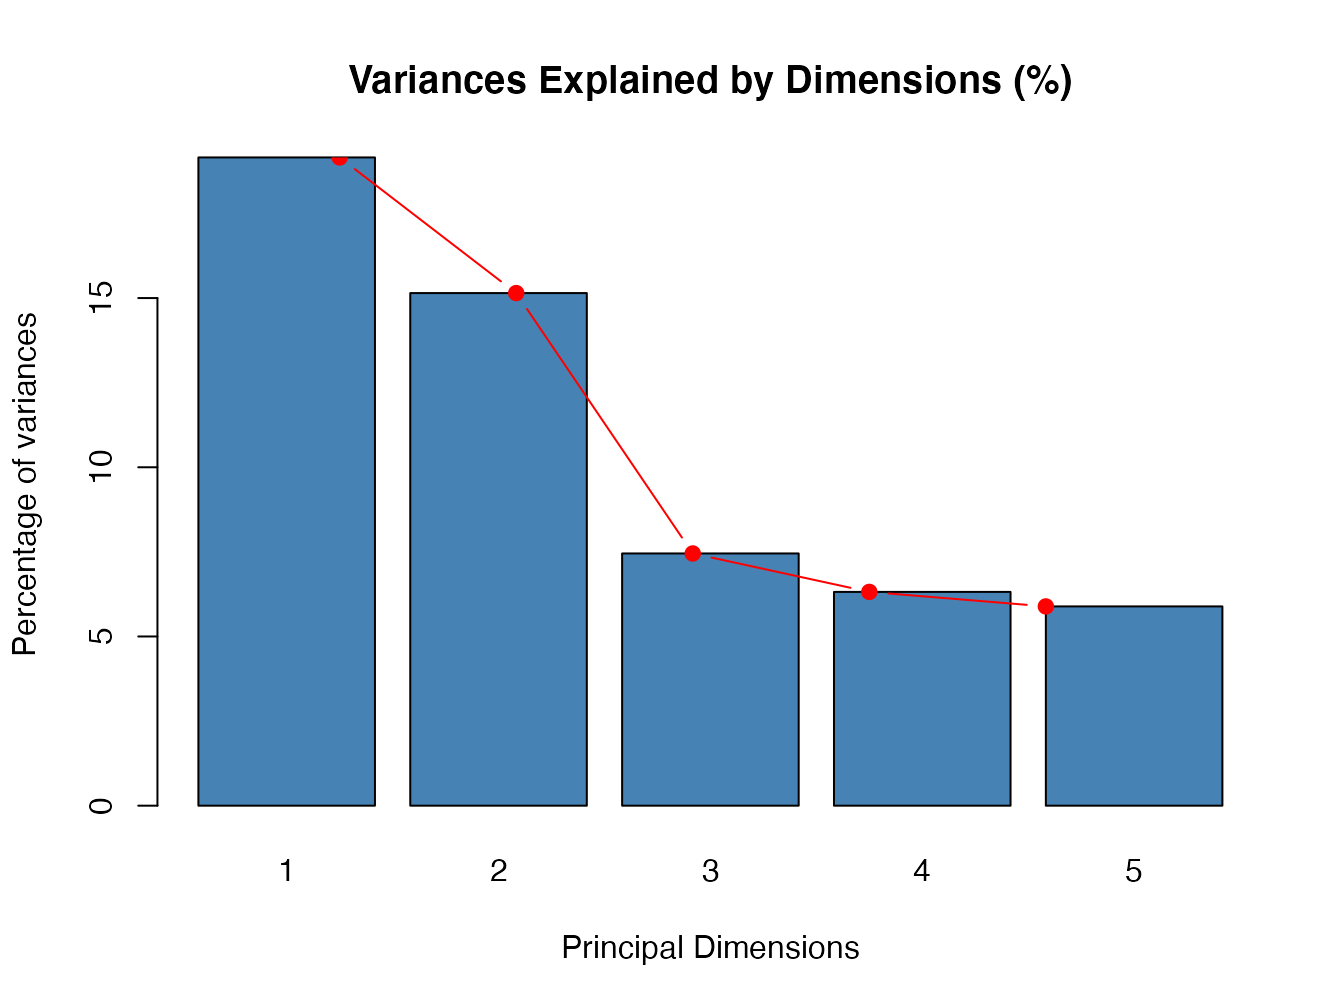
\includegraphics[width=0.8\linewidth]{MyBook_files/figure-latex/valeurs_propres-1} \end{center}

\begin{Shaded}
\begin{Highlighting}[]
\NormalTok{eig.val}
\end{Highlighting}
\end{Shaded}

\begin{verbatim}
##        eigenvalue percentage of variance
## comp 1   3.447962              19.155346
## comp 2   2.726477              15.147094
## comp 3   1.341535               7.452973
## comp 4   1.137082               6.317122
## comp 5   1.059898               5.888321
##        cumulative percentage of variance
## comp 1                          19.15535
## comp 2                          34.30244
## comp 3                          41.75541
## comp 4                          48.07254
## comp 5                          53.96086
\end{verbatim}

\normalsize

\hypertarget{toutes-les-variables}{%
\section{Toutes les variables}\label{toutes-les-variables}}

\scriptsize

\begin{Shaded}
\begin{Highlighting}[]
\NormalTok{var }\OtherTok{\textless{}{-}} \FunctionTok{get\_famd\_var}\NormalTok{(res.famd)}
\NormalTok{var}
\end{Highlighting}
\end{Shaded}

\begin{verbatim}
## FAMD results for variables 
##  ===================================================
##   Name       Description                      
## 1 "$coord"   "Coordinates"                    
## 2 "$cos2"    "Cos2, quality of representation"
## 3 "$contrib" "Contributions"
\end{verbatim}

\begin{Shaded}
\begin{Highlighting}[]
\CommentTok{\# Coordonnées des variables}
\FunctionTok{head}\NormalTok{(var}\SpecialCharTok{$}\NormalTok{coord)}
\end{Highlighting}
\end{Shaded}

\begin{verbatim}
##                   Dim.1      Dim.2        Dim.3
## diversite   0.012502394 0.02326411 0.6144465953
## n_AG        0.883183496 0.01428793 0.0128702310
## n_inf_130   0.669765802 0.05513751 0.0276744314
## n_sup_130   0.606776052 0.06560694 0.0080207337
## hauteur_moy 0.006545122 0.93612413 0.0017853949
## hauteur_min 0.029977698 0.70119872 0.0003599731
##                    Dim.4      Dim.5
## diversite   0.0009997302 0.01582323
## n_AG        0.0068694483 0.01797176
## n_inf_130   0.0066654732 0.06706463
## n_sup_130   0.0018470475 0.07582262
## hauteur_moy 0.0008132428 0.01627364
## hauteur_min 0.0011504889 0.03742157
\end{verbatim}

\begin{Shaded}
\begin{Highlighting}[]
\CommentTok{\# Cos2: qualité de représentation}
\FunctionTok{head}\NormalTok{(var}\SpecialCharTok{$}\NormalTok{cos2)}
\end{Highlighting}
\end{Shaded}

\begin{verbatim}
##                    Dim.1        Dim.2        Dim.3
## diversite   1.563098e-04 0.0005412186 3.775446e-01
## n_AG        7.800131e-01 0.0002041450 1.656428e-04
## n_inf_130   4.485862e-01 0.0030401449 7.658742e-04
## n_sup_130   3.681772e-01 0.0043042707 6.433217e-05
## hauteur_moy 4.283862e-05 0.8763283939 3.187635e-06
## hauteur_min 8.986624e-04 0.4916796414 1.295806e-07
##                    Dim.4        Dim.5
## diversite   9.994604e-07 0.0002503746
## n_AG        4.718932e-05 0.0003229840
## n_inf_130   4.442853e-05 0.0044976644
## n_sup_130   3.411585e-06 0.0057490695
## hauteur_moy 6.613638e-07 0.0002648315
## hauteur_min 1.323625e-06 0.0014003742
\end{verbatim}

\begin{Shaded}
\begin{Highlighting}[]
\CommentTok{\# Contributions aux dimensions}
\FunctionTok{head}\NormalTok{(var}\SpecialCharTok{$}\NormalTok{contrib)}
\end{Highlighting}
\end{Shaded}

\begin{verbatim}
##                  Dim.1      Dim.2       Dim.3      Dim.4
## diversite    0.3626024  0.8532662 45.80174988 0.08792067
## n_AG        25.6146512  0.5240437  0.95936588 0.60412953
## n_inf_130   19.4249750  2.0222987  2.06289268 0.58619106
## n_sup_130   17.5981061  2.4062899  0.59787725 0.16243749
## hauteur_moy  0.1898258 34.3345694  0.13308595 0.07152015
## hauteur_min  0.8694323 25.7181235  0.02683292 0.10117906
##                Dim.5
## diversite   1.492901
## n_AG        1.695612
## n_inf_130   6.327462
## n_sup_130   7.153767
## hauteur_moy 1.535397
## hauteur_min 3.530677
\end{verbatim}

\normalsize

\scriptsize

\begin{Shaded}
\begin{Highlighting}[]
\CommentTok{\# Graphique des variables}
\FunctionTok{fviz\_famd\_var}\NormalTok{(res.famd, }\AttributeTok{repel =} \ConstantTok{TRUE}\NormalTok{)}
\end{Highlighting}
\end{Shaded}

\begin{center}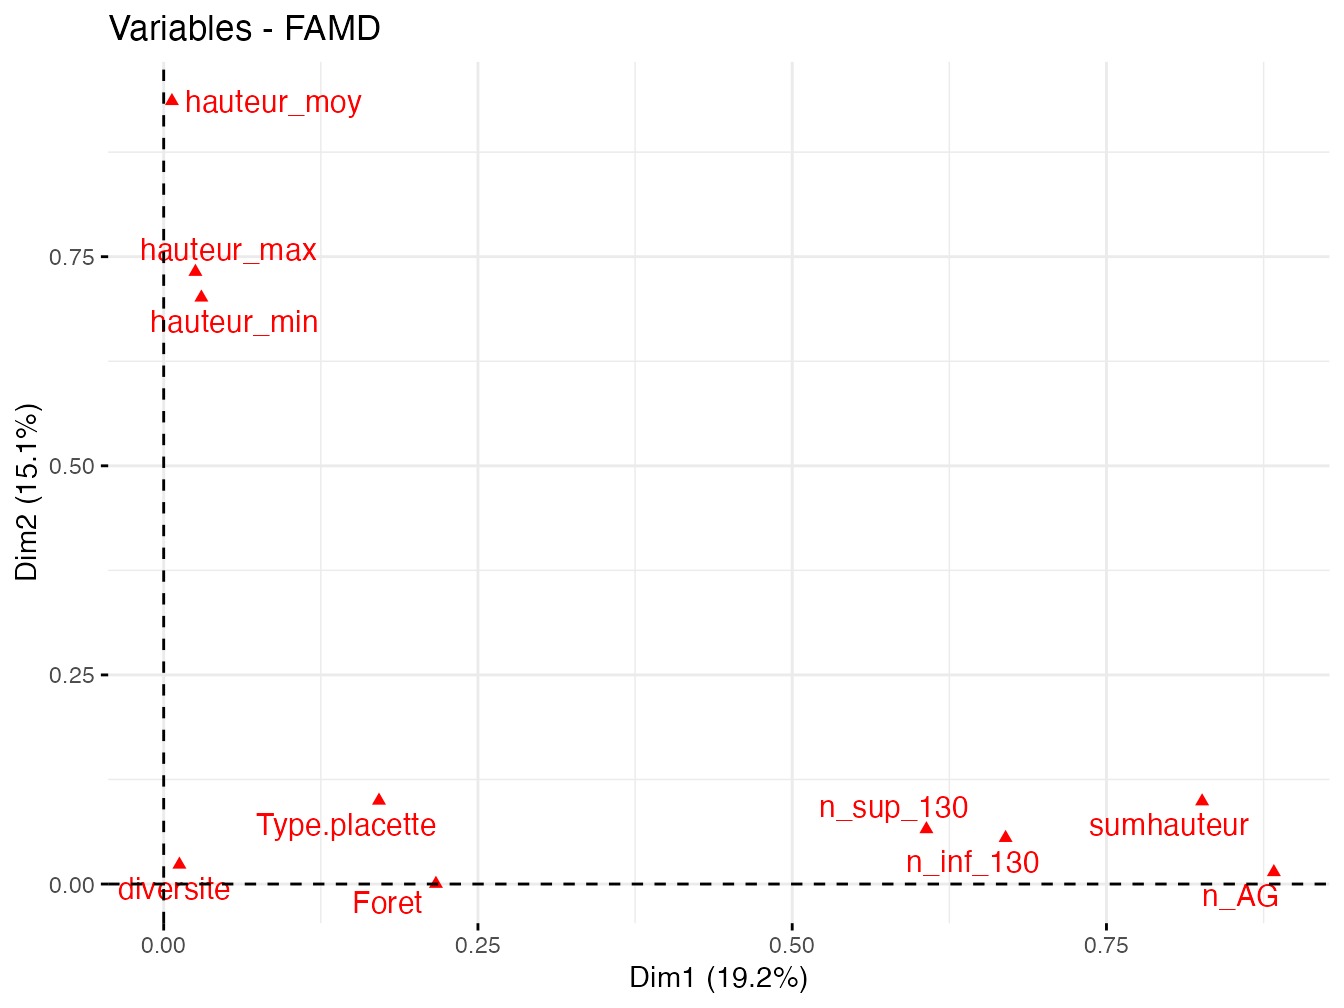
\includegraphics[width=0.8\linewidth]{MyBook_files/figure-latex/unnamed-chunk-6-1} \end{center}

\begin{Shaded}
\begin{Highlighting}[]
\FunctionTok{fviz\_famd\_var}\NormalTok{(res.famd, }\AttributeTok{repel =} \ConstantTok{TRUE}\NormalTok{)}
\end{Highlighting}
\end{Shaded}

\begin{center}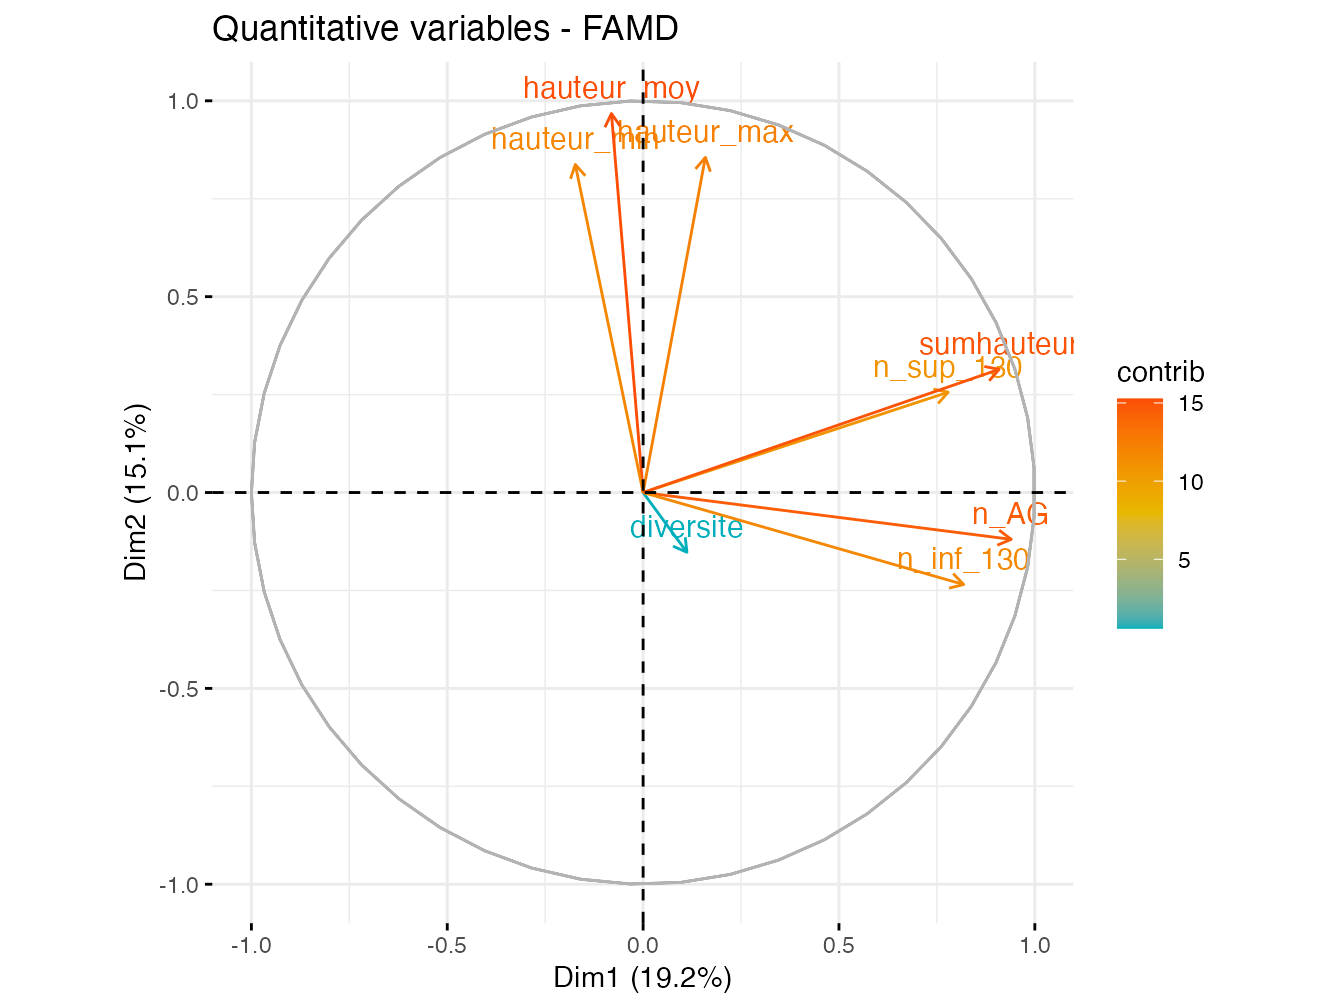
\includegraphics[width=0.8\linewidth]{MyBook_files/figure-latex/unnamed-chunk-6-2} \end{center}

\begin{Shaded}
\begin{Highlighting}[]
\CommentTok{\# Contribution à la première dimension}
\FunctionTok{fviz\_contrib}\NormalTok{(res.famd, }\StringTok{"var"}\NormalTok{, }\AttributeTok{axes =} \DecValTok{1}\NormalTok{)}
\end{Highlighting}
\end{Shaded}

\begin{center}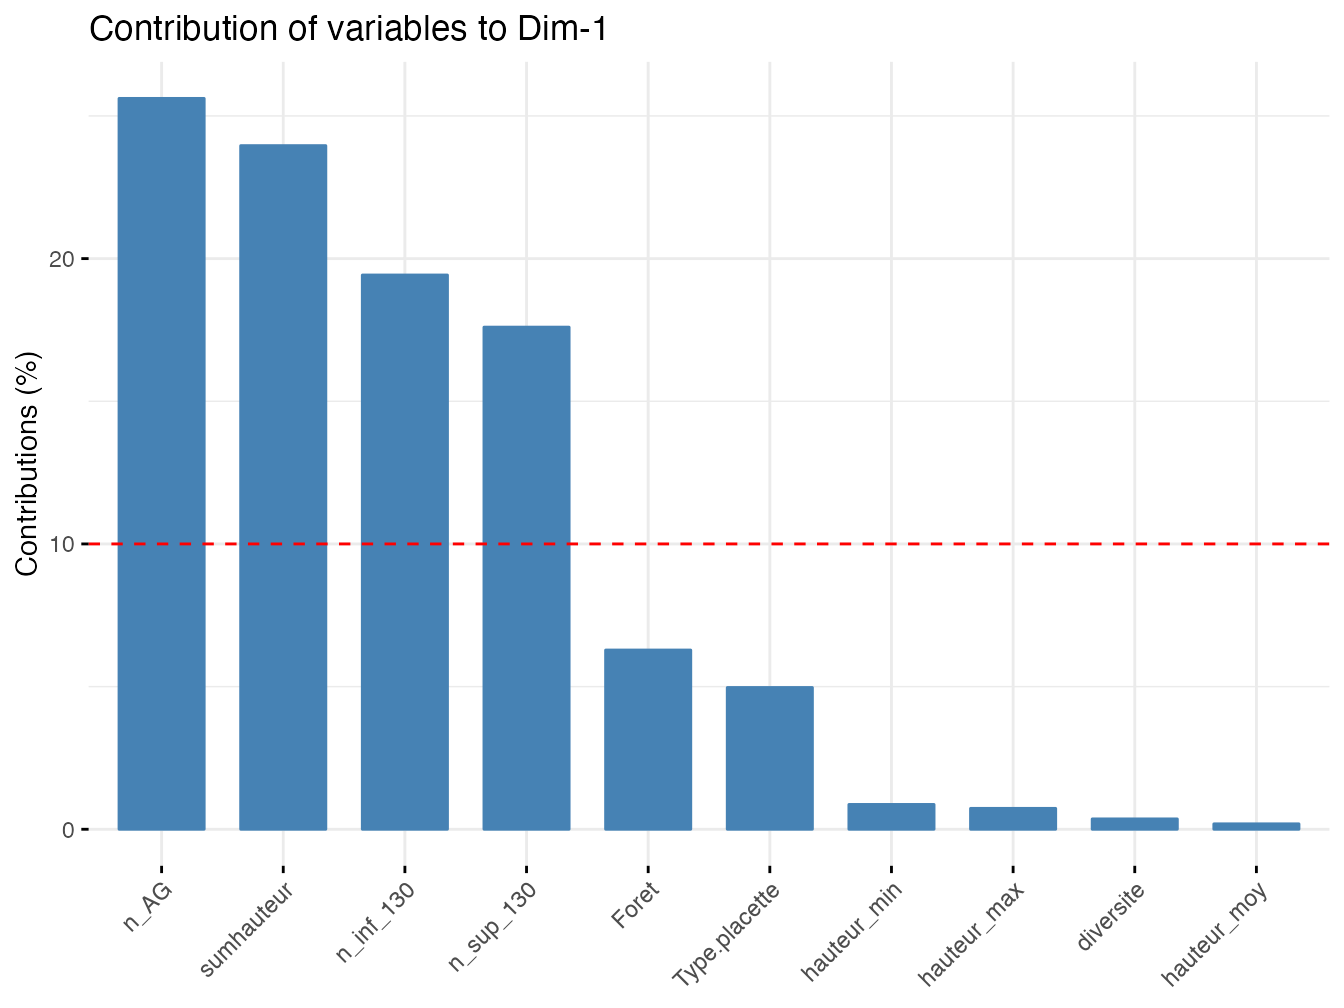
\includegraphics[width=0.8\linewidth]{MyBook_files/figure-latex/unnamed-chunk-6-3} \end{center}

\begin{Shaded}
\begin{Highlighting}[]
\CommentTok{\# Contribution à la deuxième dimension}
\FunctionTok{fviz\_contrib}\NormalTok{(res.famd, }\StringTok{"var"}\NormalTok{, }\AttributeTok{axes =} \DecValTok{2}\NormalTok{)}
\end{Highlighting}
\end{Shaded}

\begin{center}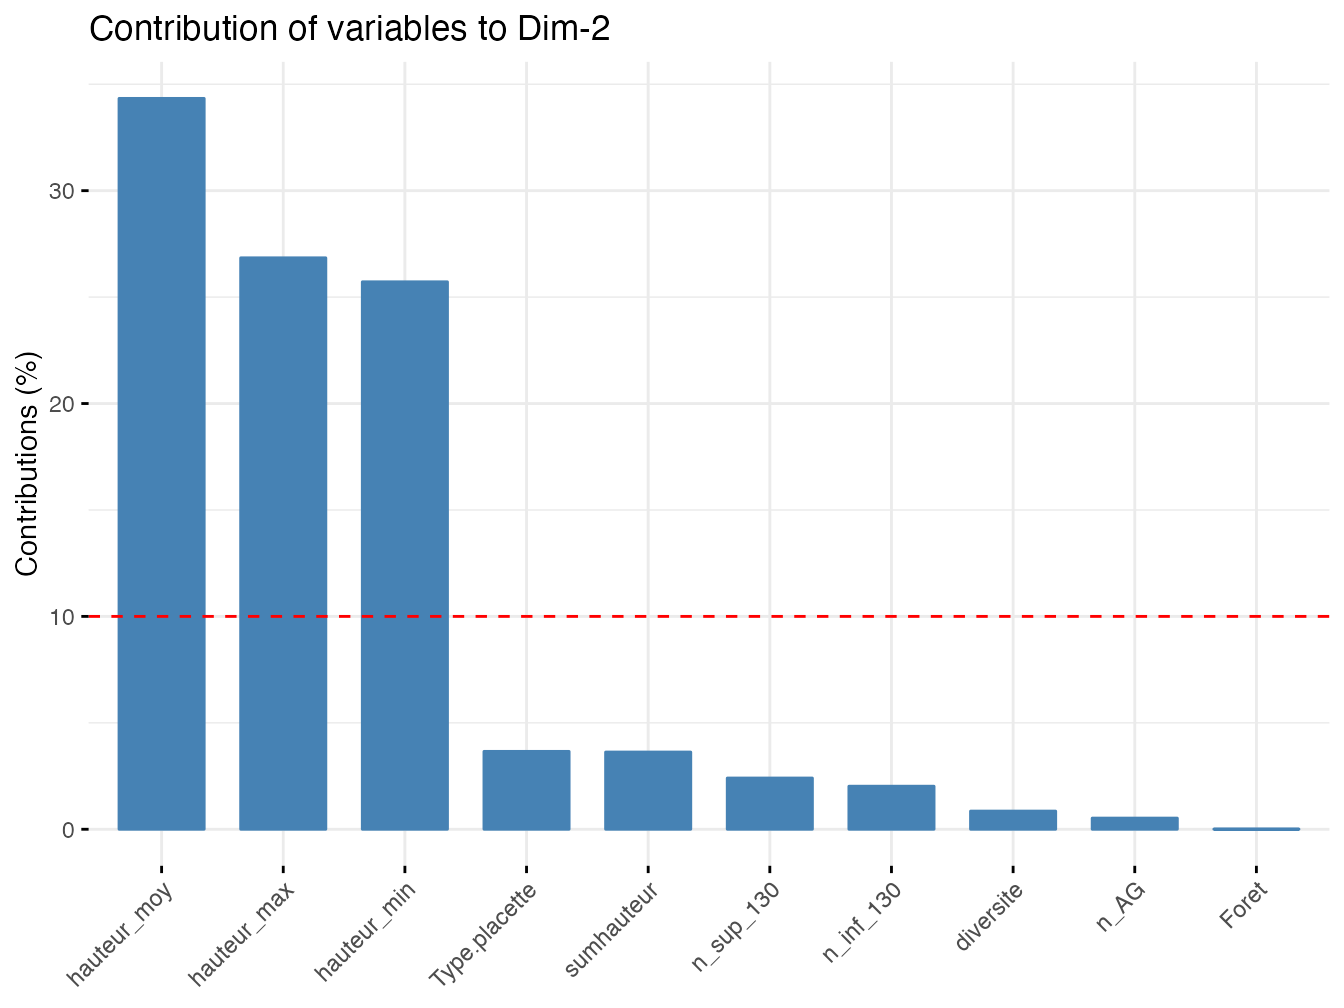
\includegraphics[width=0.8\linewidth]{MyBook_files/figure-latex/unnamed-chunk-6-4} \end{center}

\begin{Shaded}
\begin{Highlighting}[]
\CommentTok{\# Contribution à la 3e dimension}
\FunctionTok{fviz\_contrib}\NormalTok{(res.famd, }\StringTok{"var"}\NormalTok{, }\AttributeTok{axes =} \DecValTok{3}\NormalTok{)}
\end{Highlighting}
\end{Shaded}

\begin{center}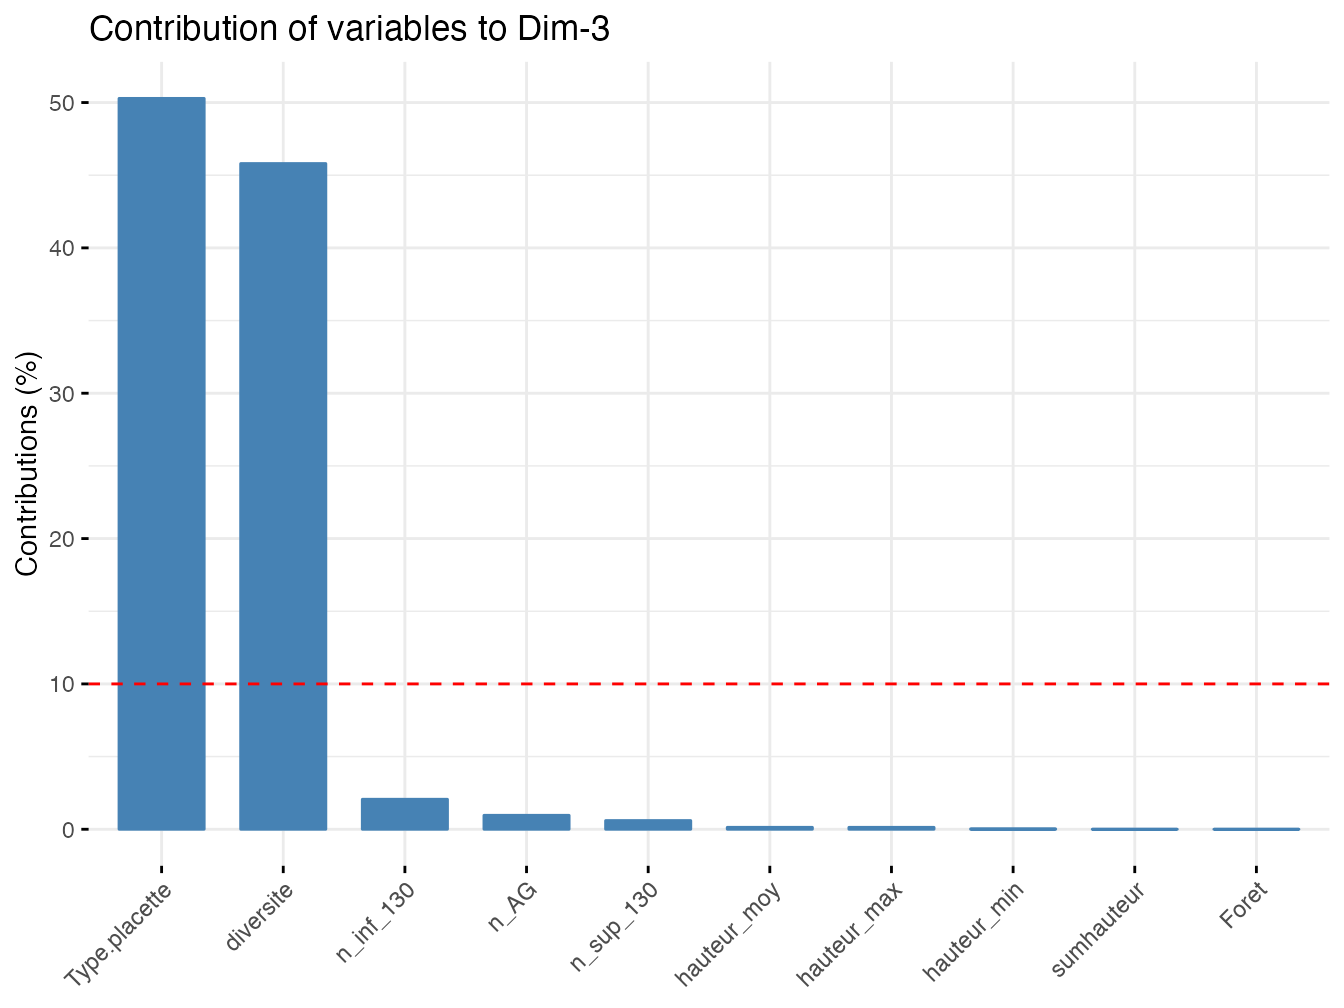
\includegraphics[width=0.8\linewidth]{MyBook_files/figure-latex/unnamed-chunk-6-5} \end{center}

\normalsize

\#\#Variables quantitatives

\scriptsize

\begin{Shaded}
\begin{Highlighting}[]
\NormalTok{quanti.var }\OtherTok{\textless{}{-}} \FunctionTok{get\_famd\_var}\NormalTok{(res.famd, }\StringTok{"quanti.var"}\NormalTok{)}
\NormalTok{quanti.var}
\end{Highlighting}
\end{Shaded}

\begin{verbatim}
## FAMD results for quantitative variables 
##  ===================================================
##   Name       Description                      
## 1 "$coord"   "Coordinates"                    
## 2 "$cos2"    "Cos2, quality of representation"
## 3 "$contrib" "Contributions"
\end{verbatim}

\begin{Shaded}
\begin{Highlighting}[]
\FunctionTok{fviz\_famd\_var}\NormalTok{(res.famd, }\StringTok{"quanti.var"}\NormalTok{, }\AttributeTok{col.var =} \StringTok{"black"}\NormalTok{)  }\CommentTok{\# on ne peut pas utiliser repel=TRUE car trop de variables}
\end{Highlighting}
\end{Shaded}

\begin{center}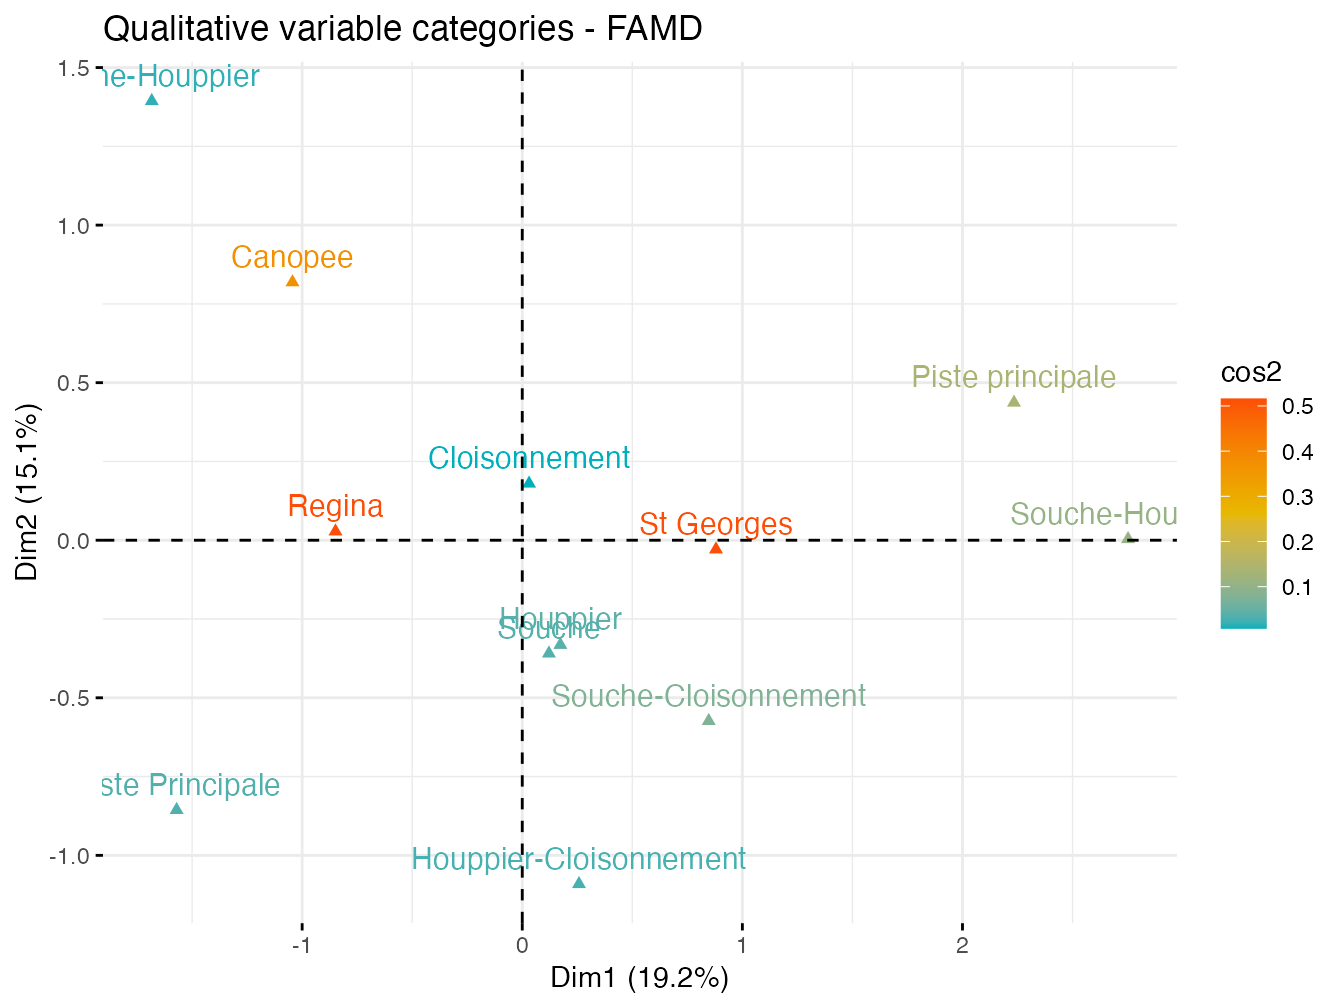
\includegraphics[width=0.8\linewidth]{MyBook_files/figure-latex/unnamed-chunk-7-1} \end{center}

\begin{Shaded}
\begin{Highlighting}[]
\CommentTok{\# fviz\_famd\_var(res.famd, \textquotesingle{}quanti.var\textquotesingle{}, repel =}
\CommentTok{\# TRUE,col.var = \textquotesingle{}black\textquotesingle{})}
\CommentTok{\# couleur selon importance de la contribution aux axes}
\FunctionTok{fviz\_famd\_var}\NormalTok{(res.famd, }\StringTok{"quanti.var"}\NormalTok{, }\AttributeTok{col.var =} \StringTok{"contrib"}\NormalTok{, }\AttributeTok{gradient.cols =} \FunctionTok{c}\NormalTok{(}\StringTok{"\#00AFBB"}\NormalTok{,}
    \StringTok{"\#E7B800"}\NormalTok{, }\StringTok{"\#FC4E07"}\NormalTok{))}
\end{Highlighting}
\end{Shaded}

\begin{center}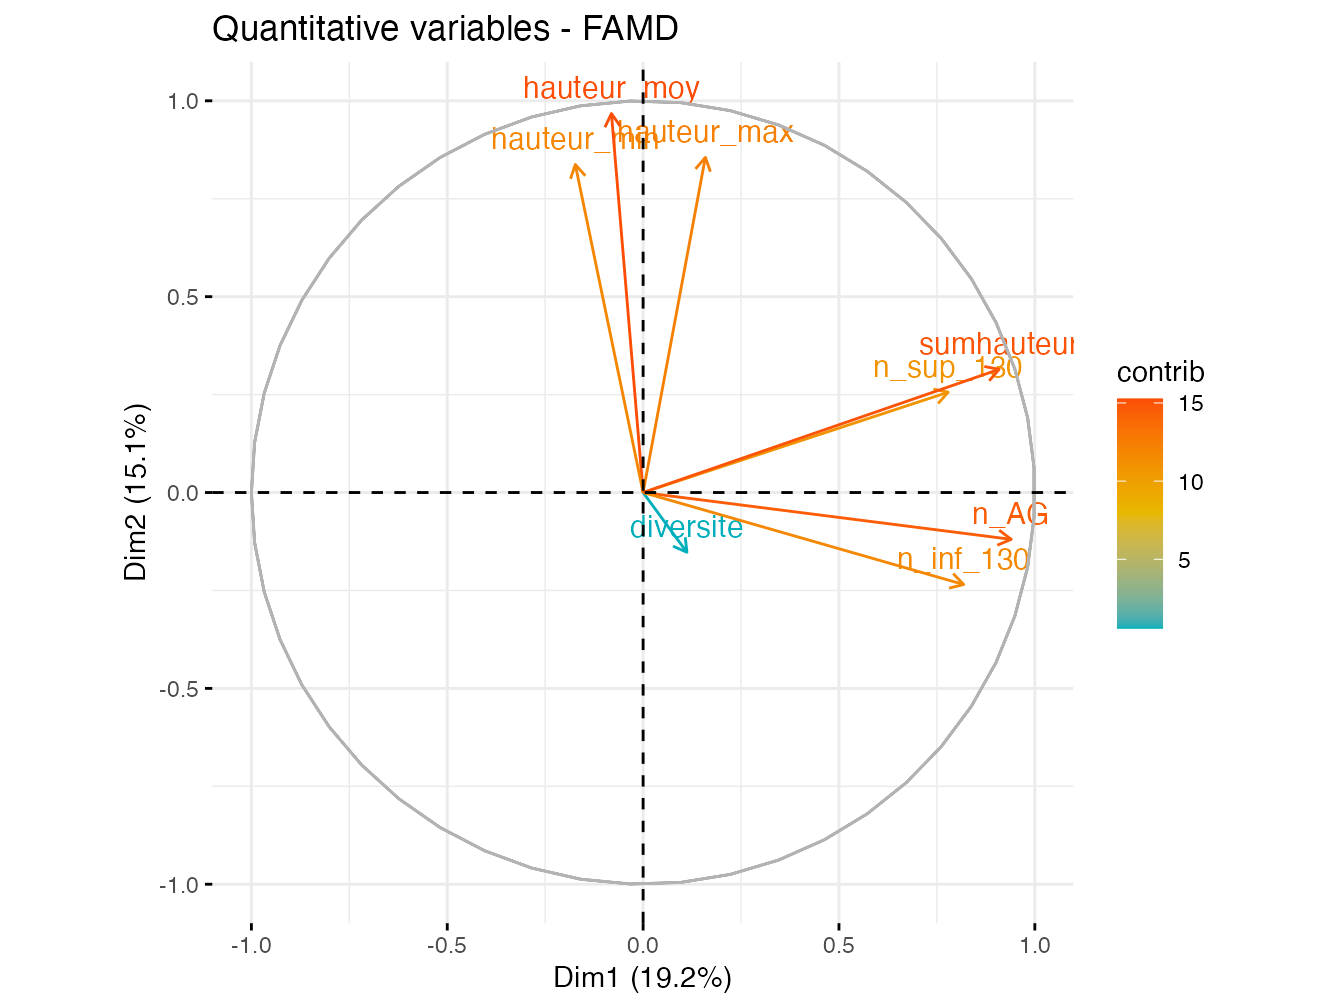
\includegraphics[width=0.8\linewidth]{MyBook_files/figure-latex/unnamed-chunk-7-2} \end{center}

\begin{Shaded}
\begin{Highlighting}[]
\CommentTok{\# Couleur par valeurs cos2: qualité sur le plan des}
\CommentTok{\# facteurs}
\FunctionTok{fviz\_famd\_var}\NormalTok{(res.famd, }\StringTok{"quanti.var"}\NormalTok{, }\AttributeTok{col.var =} \StringTok{"cos2"}\NormalTok{, }\AttributeTok{gradient.cols =} \FunctionTok{c}\NormalTok{(}\StringTok{"\#00AFBB"}\NormalTok{,}
    \StringTok{"\#E7B800"}\NormalTok{, }\StringTok{"\#FC4E07"}\NormalTok{))}
\end{Highlighting}
\end{Shaded}

\begin{center}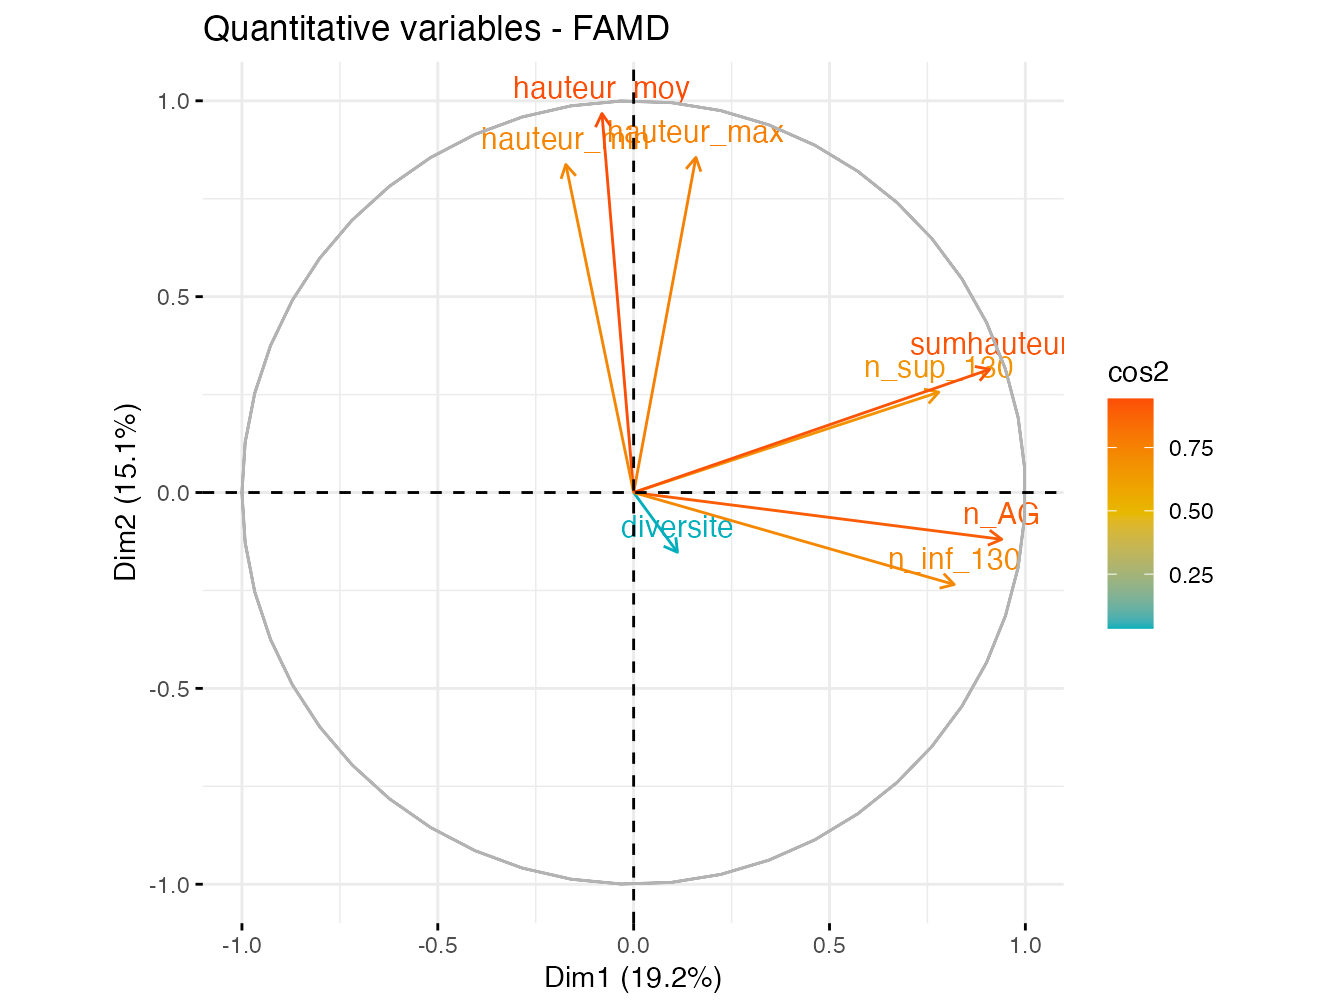
\includegraphics[width=0.8\linewidth]{MyBook_files/figure-latex/unnamed-chunk-7-3} \end{center}

\begin{Shaded}
\begin{Highlighting}[]
\FunctionTok{fviz\_famd\_var}\NormalTok{(res.famd, }\StringTok{"quanti.var"}\NormalTok{, }\AttributeTok{col.var =} \StringTok{"cos2"}\NormalTok{, }\AttributeTok{gradient.cols =} \FunctionTok{c}\NormalTok{(}\StringTok{"\#00AFBB"}\NormalTok{,}
    \StringTok{"\#E7B800"}\NormalTok{, }\StringTok{"\#FC4E07"}\NormalTok{), }\AttributeTok{axes =} \FunctionTok{c}\NormalTok{(}\DecValTok{1}\NormalTok{, }\DecValTok{3}\NormalTok{))}
\end{Highlighting}
\end{Shaded}

\begin{center}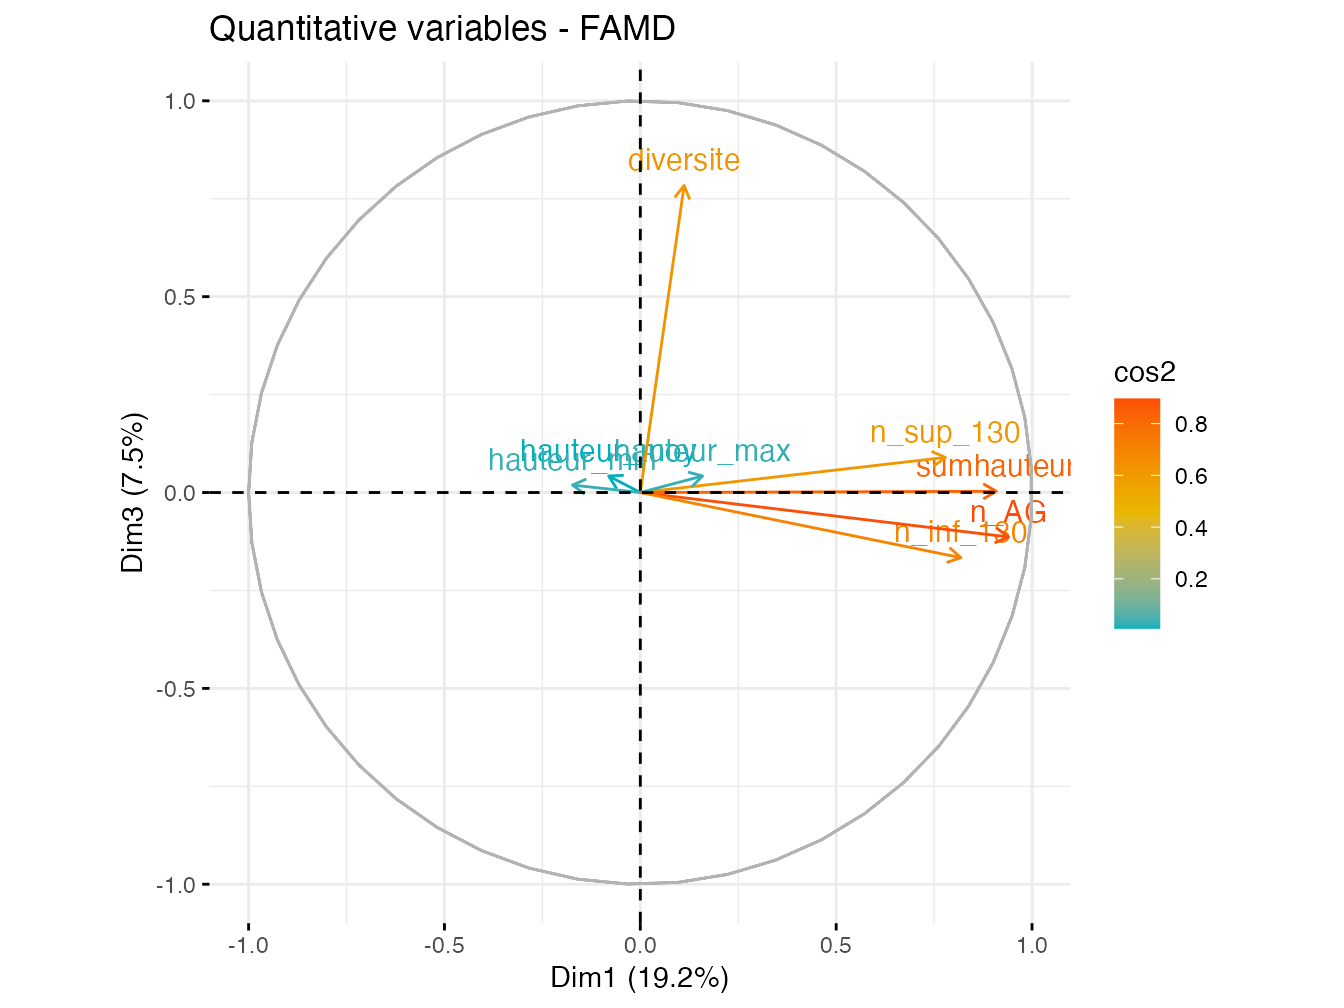
\includegraphics[width=0.8\linewidth]{MyBook_files/figure-latex/unnamed-chunk-7-4} \end{center}

\begin{Shaded}
\begin{Highlighting}[]
\CommentTok{\# Cos2 total des variables sur Dim.1 et Dim.2}
\FunctionTok{fviz\_cos2}\NormalTok{(res.famd, }\AttributeTok{choice =} \StringTok{"var"}\NormalTok{, }\AttributeTok{axes =} \DecValTok{1}\SpecialCharTok{:}\DecValTok{2}\NormalTok{)}
\end{Highlighting}
\end{Shaded}

\begin{center}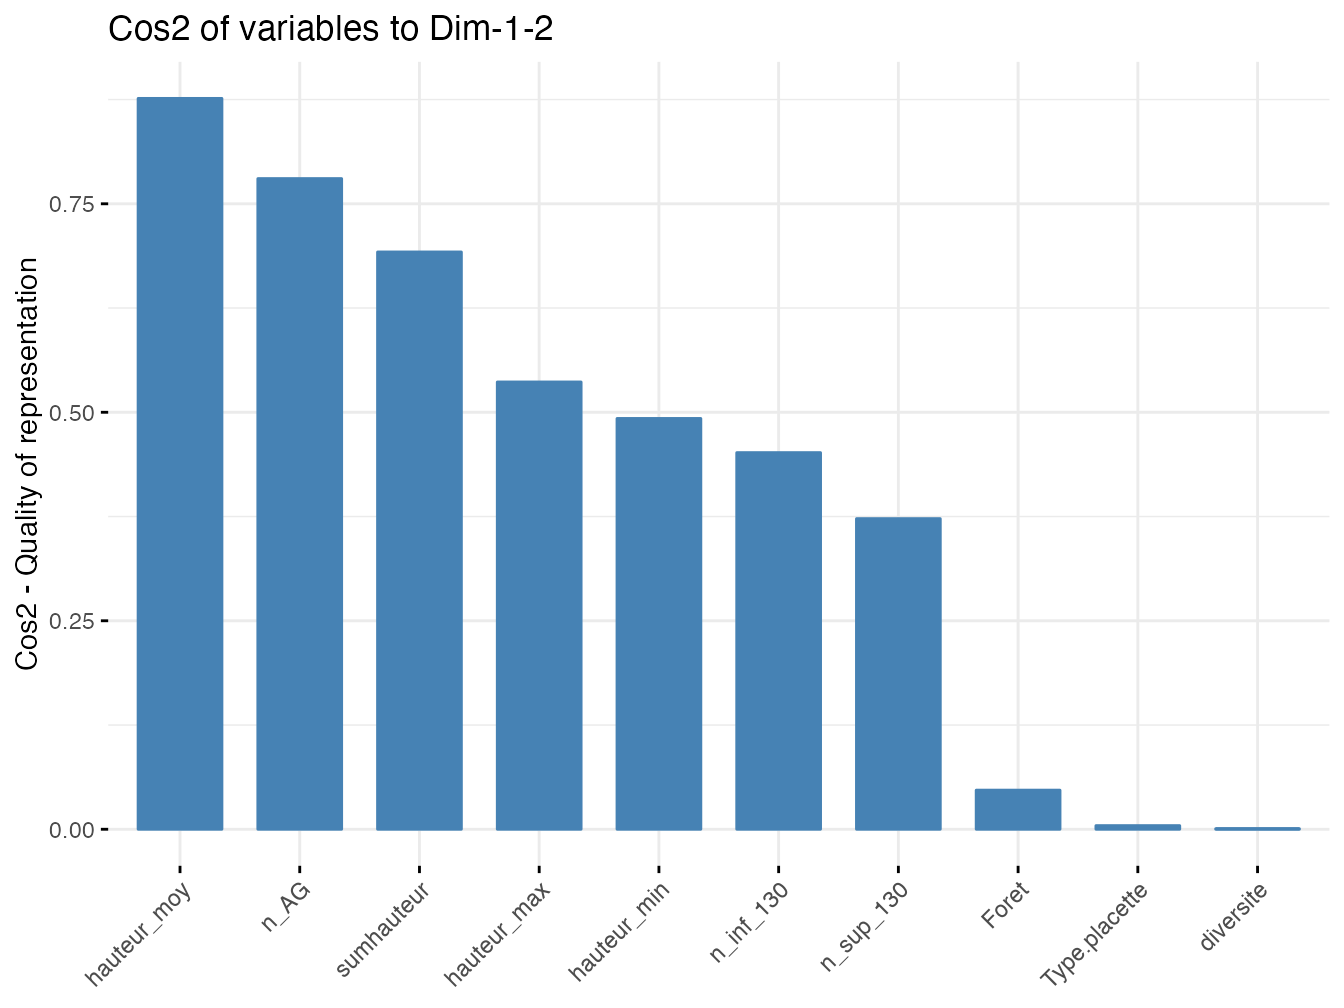
\includegraphics[width=0.8\linewidth]{MyBook_files/figure-latex/unnamed-chunk-7-5} \end{center}

\begin{Shaded}
\begin{Highlighting}[]
\CommentTok{\# Cos2 total des variables sur Dim.1 et Dim.3}
\FunctionTok{fviz\_cos2}\NormalTok{(res.famd, }\AttributeTok{choice =} \StringTok{"var"}\NormalTok{, }\AttributeTok{axes =} \DecValTok{1}\SpecialCharTok{:}\DecValTok{3}\NormalTok{)}
\end{Highlighting}
\end{Shaded}

\begin{center}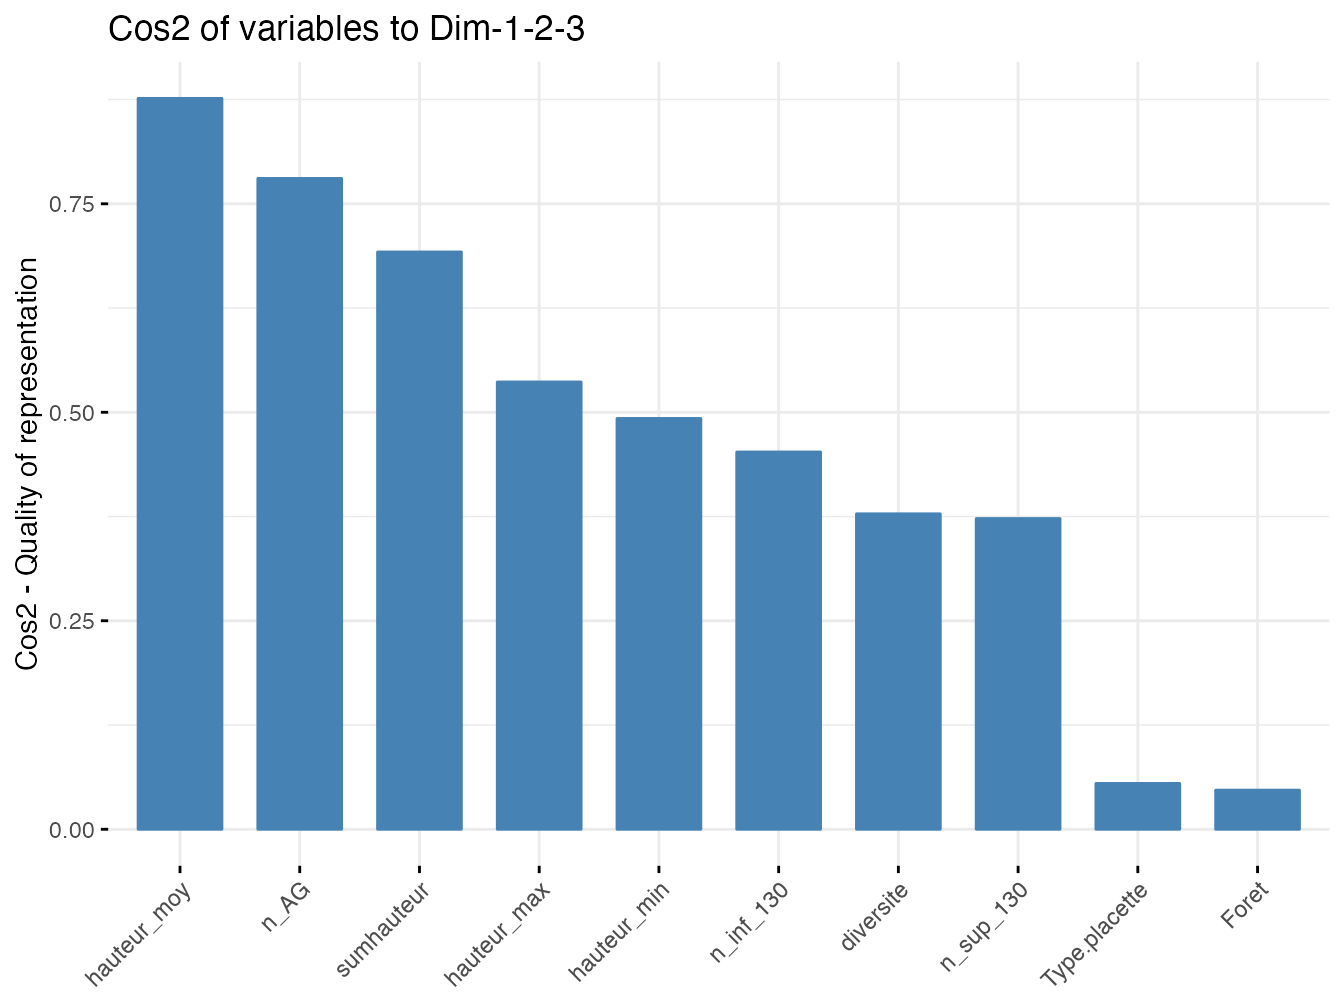
\includegraphics[width=0.8\linewidth]{MyBook_files/figure-latex/unnamed-chunk-7-6} \end{center}

\normalsize

\#\#Variables qualitatives

\scriptsize

\begin{Shaded}
\begin{Highlighting}[]
\NormalTok{quali.var }\OtherTok{\textless{}{-}} \FunctionTok{get\_famd\_var}\NormalTok{(res.famd, }\StringTok{"quali.var"}\NormalTok{)}
\NormalTok{quali.var}
\end{Highlighting}
\end{Shaded}

\begin{verbatim}
## FAMD results for qualitative variable categories 
##  ===================================================
##   Name       Description                      
## 1 "$coord"   "Coordinates"                    
## 2 "$cos2"    "Cos2, quality of representation"
## 3 "$contrib" "Contributions"
\end{verbatim}

\begin{Shaded}
\begin{Highlighting}[]
\FunctionTok{fviz\_famd\_var}\NormalTok{(res.famd, }\StringTok{"quali.var"}\NormalTok{, }\AttributeTok{col.var =} \StringTok{"cos2"}\NormalTok{, }\AttributeTok{gradient.cols =} \FunctionTok{c}\NormalTok{(}\StringTok{"\#00AFBB"}\NormalTok{,}
    \StringTok{"\#E7B800"}\NormalTok{, }\StringTok{"\#FC4E07"}\NormalTok{))}
\end{Highlighting}
\end{Shaded}

\begin{center}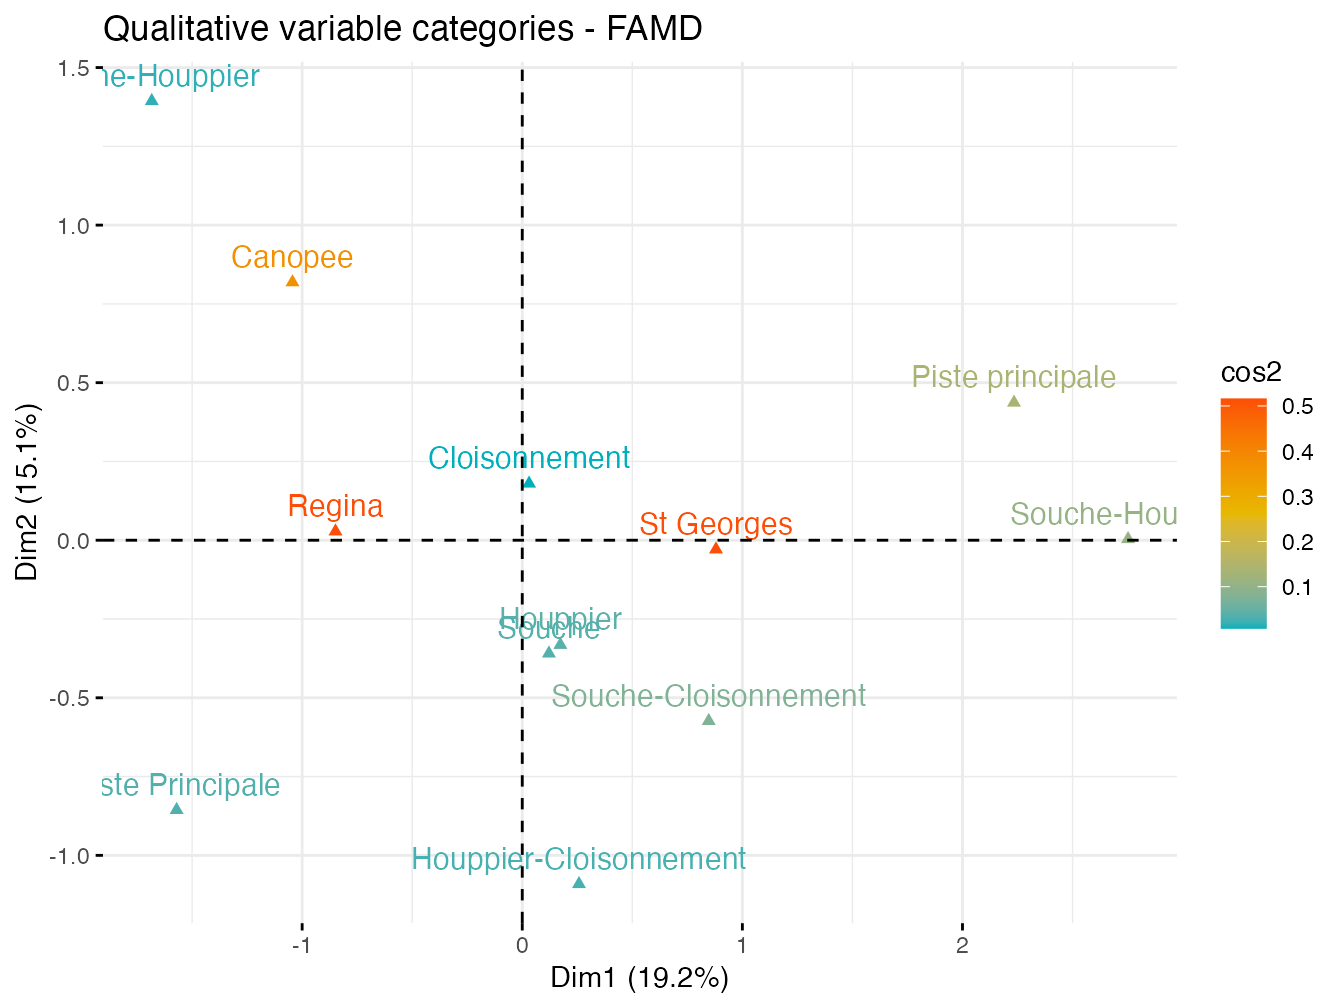
\includegraphics[width=0.8\linewidth]{MyBook_files/figure-latex/unnamed-chunk-8-1} \end{center}

\begin{Shaded}
\begin{Highlighting}[]
\FunctionTok{fviz\_famd\_var}\NormalTok{(res.famd, }\StringTok{"quali.var"}\NormalTok{, }\AttributeTok{col.var =} \StringTok{"cos2"}\NormalTok{, }\AttributeTok{gradient.cols =} \FunctionTok{c}\NormalTok{(}\StringTok{"\#00AFBB"}\NormalTok{,}
    \StringTok{"\#E7B800"}\NormalTok{, }\StringTok{"\#FC4E07"}\NormalTok{), }\AttributeTok{axes =} \FunctionTok{c}\NormalTok{(}\DecValTok{1}\NormalTok{, }\DecValTok{3}\NormalTok{))}
\end{Highlighting}
\end{Shaded}

\begin{center}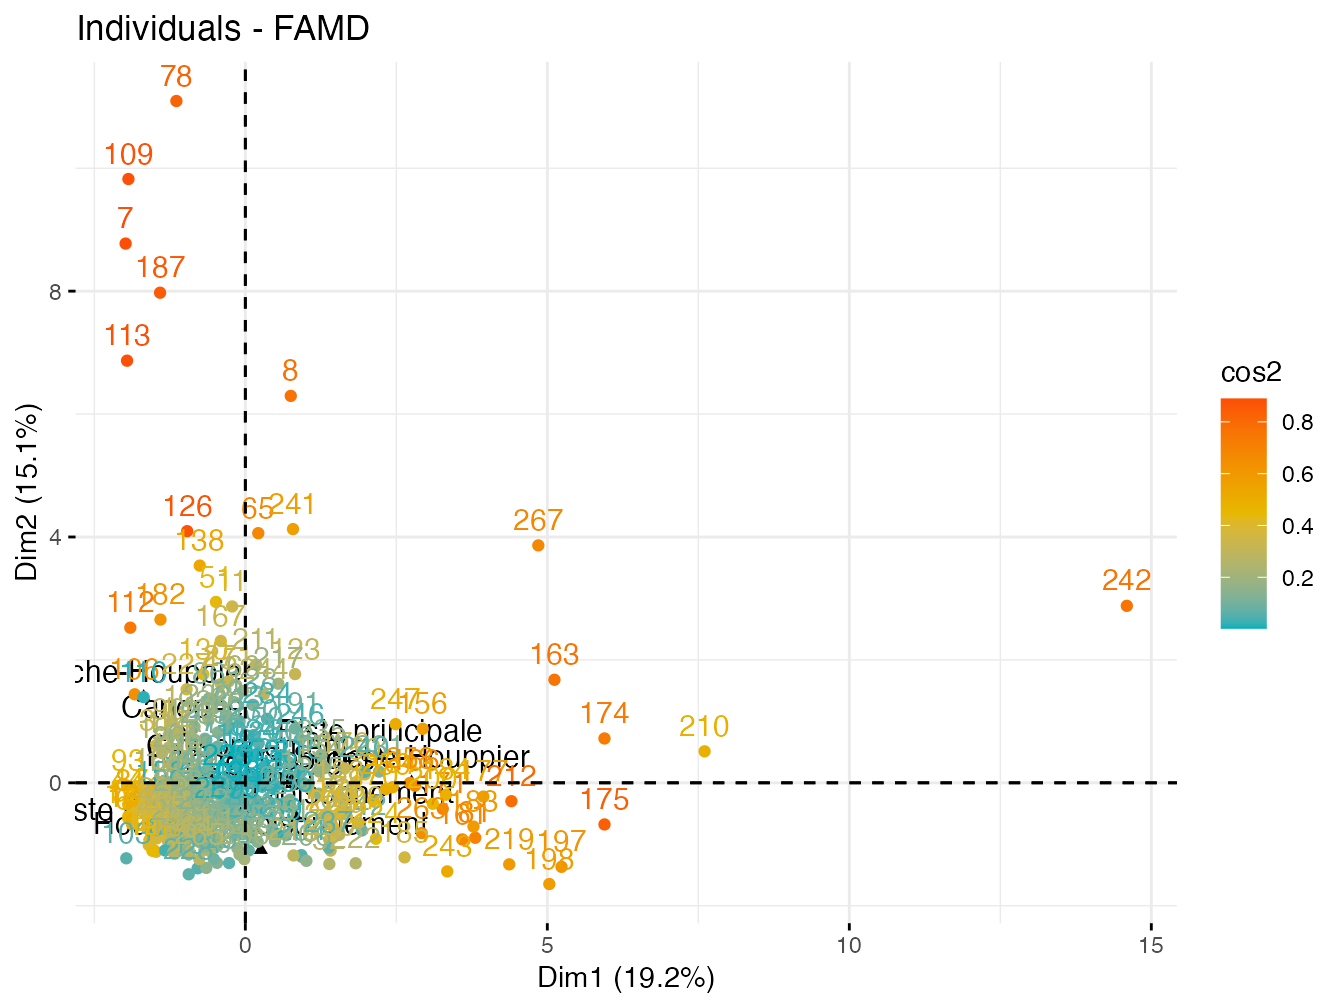
\includegraphics[width=0.8\linewidth]{MyBook_files/figure-latex/unnamed-chunk-8-2} \end{center}

\normalsize

\#\#Individus

\scriptsize

\begin{Shaded}
\begin{Highlighting}[]
\NormalTok{ind }\OtherTok{\textless{}{-}} \FunctionTok{get\_famd\_ind}\NormalTok{(res.famd)}
\NormalTok{ind}
\end{Highlighting}
\end{Shaded}

\begin{verbatim}
## FAMD results for individuals 
##  ===================================================
##   Name       Description                      
## 1 "$coord"   "Coordinates"                    
## 2 "$cos2"    "Cos2, quality of representation"
## 3 "$contrib" "Contributions"
\end{verbatim}

\begin{Shaded}
\begin{Highlighting}[]
\CommentTok{\#couleur par contribution aux axes}
\FunctionTok{fviz\_famd\_ind}\NormalTok{(res.famd, }\AttributeTok{col.ind =} \StringTok{"contrib"}\NormalTok{,}
             \AttributeTok{gradient.cols =} \FunctionTok{c}\NormalTok{(}\StringTok{"\#00AFBB"}\NormalTok{, }\StringTok{"\#E7B800"}\NormalTok{, }\StringTok{"\#FC4E07"}\NormalTok{))}
\end{Highlighting}
\end{Shaded}

\begin{center}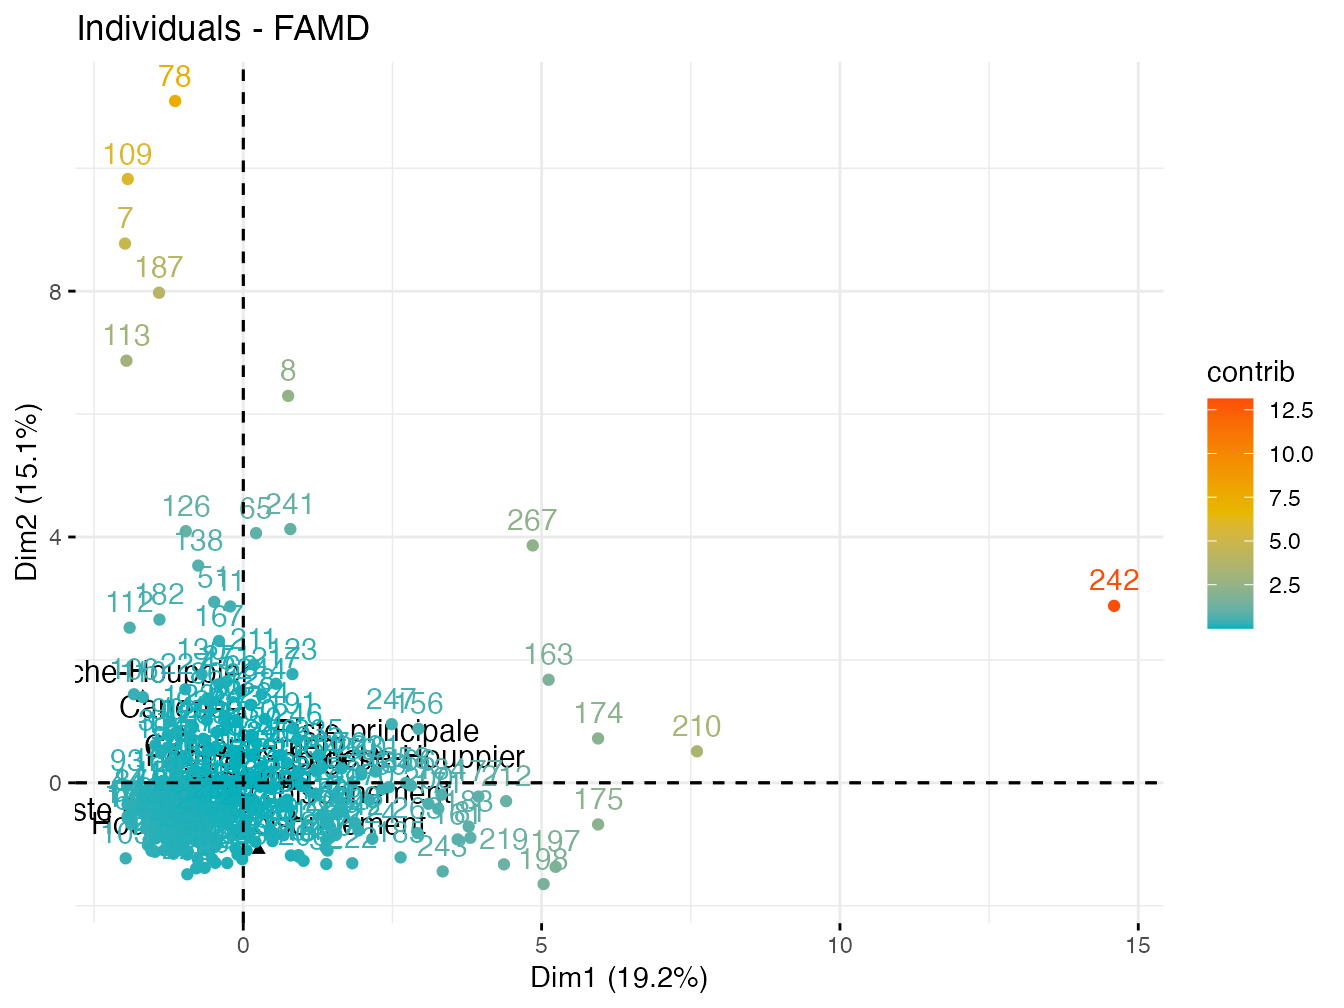
\includegraphics[width=0.8\linewidth]{MyBook_files/figure-latex/unnamed-chunk-9-1} \end{center}

\begin{Shaded}
\begin{Highlighting}[]
\CommentTok{\#couleur par qualité de representation}
\FunctionTok{fviz\_famd\_ind}\NormalTok{(res.famd, }\AttributeTok{col.ind =} \StringTok{"cos2"}\NormalTok{,}
             \AttributeTok{gradient.cols =} \FunctionTok{c}\NormalTok{(}\StringTok{"\#00AFBB"}\NormalTok{, }\StringTok{"\#E7B800"}\NormalTok{, }\StringTok{"\#FC4E07"}\NormalTok{))}
\end{Highlighting}
\end{Shaded}

\begin{center}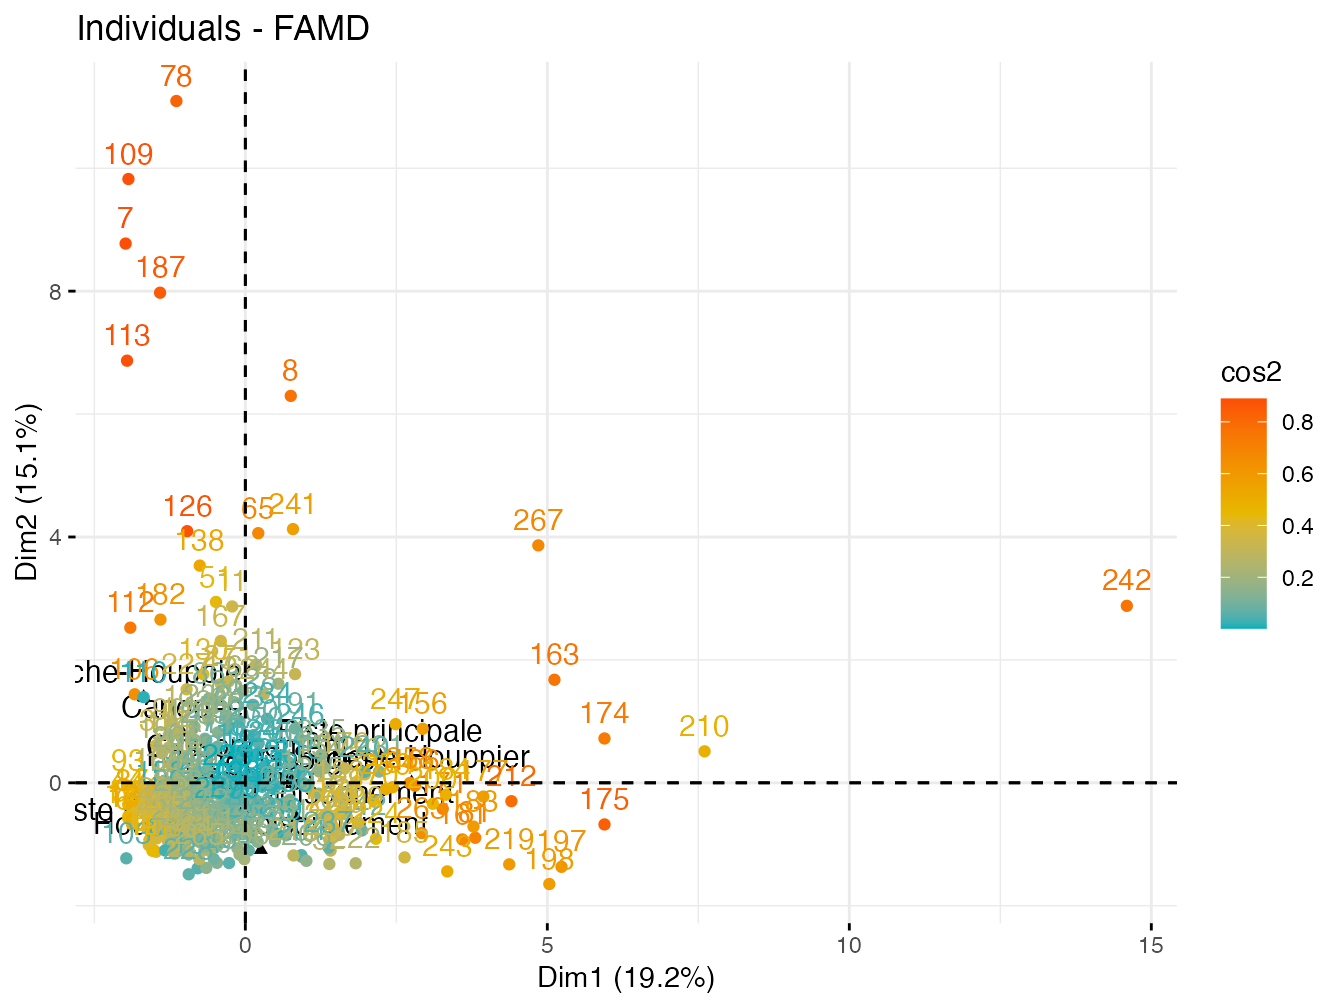
\includegraphics[width=0.8\linewidth]{MyBook_files/figure-latex/unnamed-chunk-9-2} \end{center}

\begin{Shaded}
\begin{Highlighting}[]
\CommentTok{\#couleur par traitement}
\FunctionTok{fviz\_mfa\_ind}\NormalTok{(res.famd, }
             \AttributeTok{habillage =} \StringTok{"Foret"}\NormalTok{, }\CommentTok{\# color by groups }
             \AttributeTok{palette =} \FunctionTok{c}\NormalTok{(}\StringTok{"\#00AFBB"}\NormalTok{, }\StringTok{"\#E7B800"}\NormalTok{, }\StringTok{"\#FC4E07"}\NormalTok{),}
             \AttributeTok{addEllipses =} \ConstantTok{TRUE}\NormalTok{, }\AttributeTok{ellipse.type =} \StringTok{"confidence"}\NormalTok{, }
             \AttributeTok{repel =} \ConstantTok{TRUE} \CommentTok{\# Avoid text overlapping}
\NormalTok{             ) }
\end{Highlighting}
\end{Shaded}

\begin{center}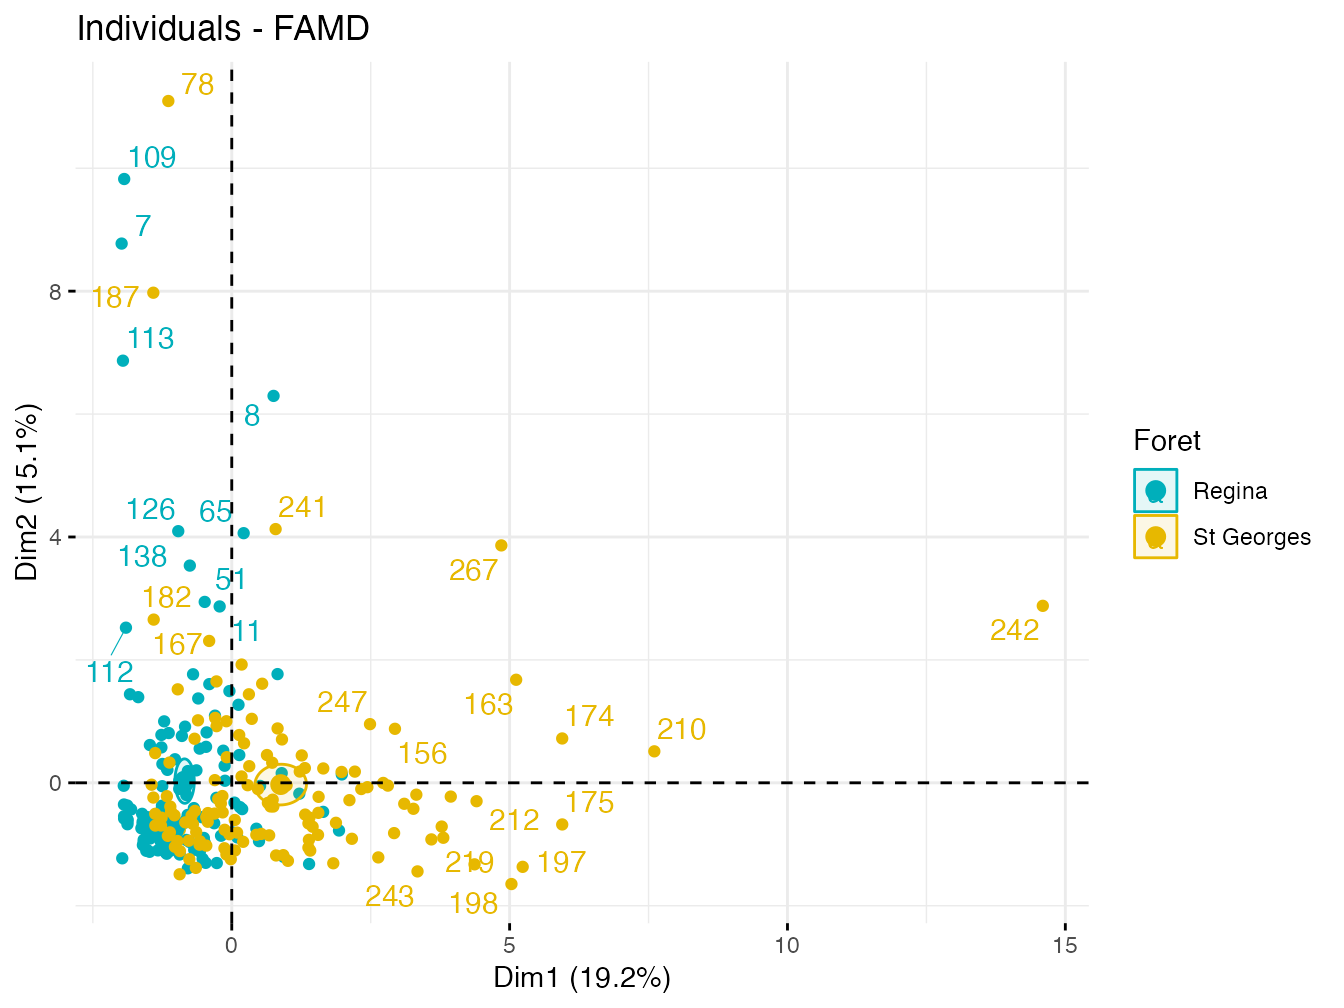
\includegraphics[width=0.8\linewidth]{MyBook_files/figure-latex/unnamed-chunk-9-3} \end{center}

\begin{Shaded}
\begin{Highlighting}[]
\FunctionTok{fviz\_ellipses}\NormalTok{(res.famd, }\FunctionTok{c}\NormalTok{(}\StringTok{"Foret"}\NormalTok{))}
\end{Highlighting}
\end{Shaded}

\begin{center}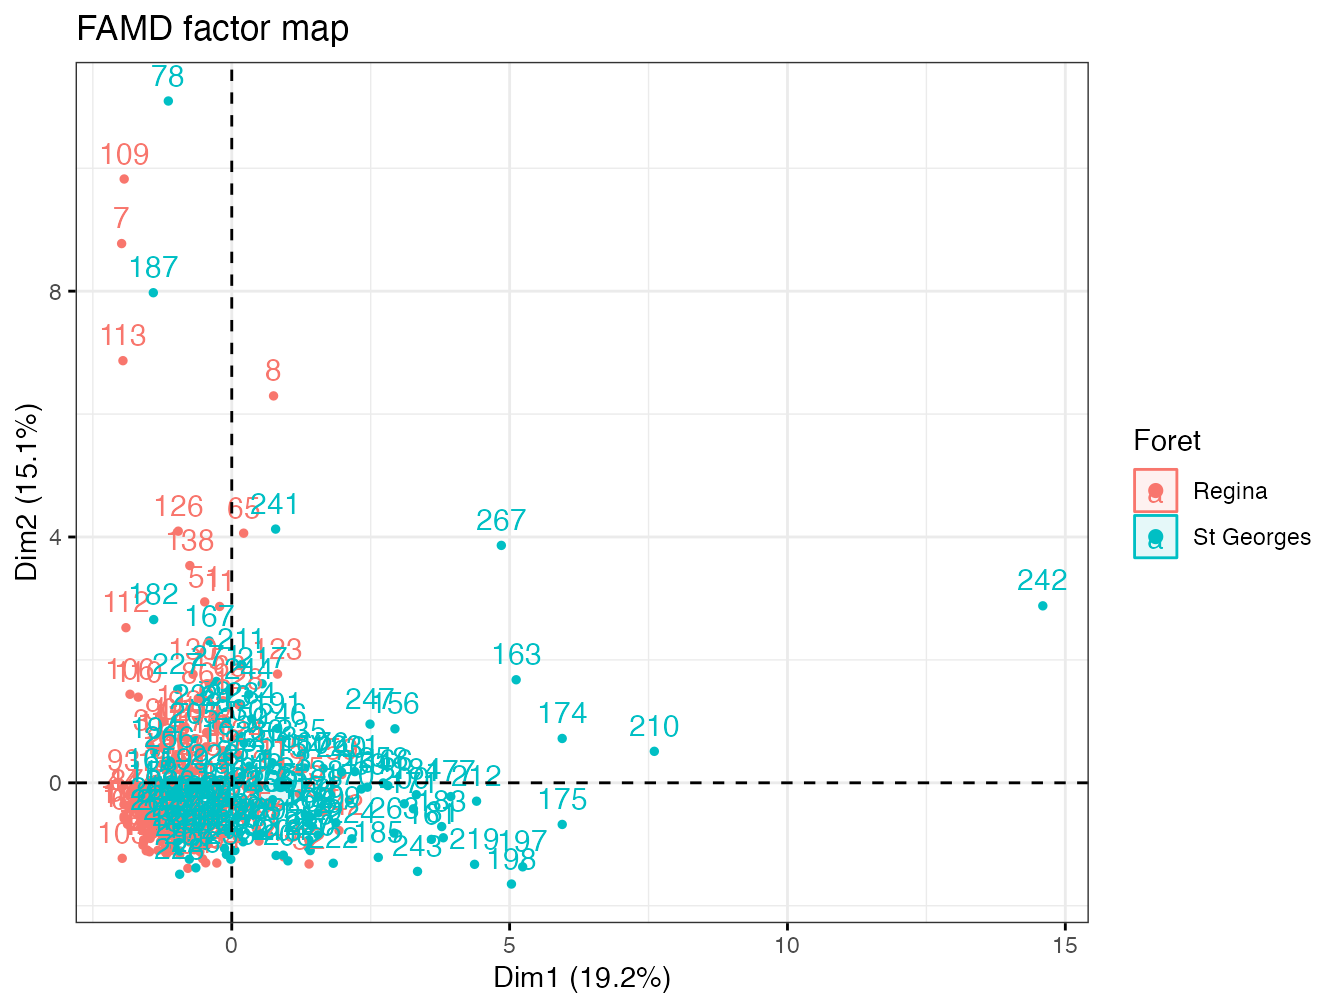
\includegraphics[width=0.8\linewidth]{MyBook_files/figure-latex/unnamed-chunk-9-4} \end{center}

\begin{Shaded}
\begin{Highlighting}[]
\CommentTok{\# n\textquotesingle{}affiche pas le num des individus}
\FunctionTok{fviz\_ellipses}\NormalTok{(res.famd, }\DecValTok{1}\SpecialCharTok{:}\DecValTok{2}\NormalTok{, }\AttributeTok{geom =} \StringTok{"point"}\NormalTok{)}
\end{Highlighting}
\end{Shaded}

\begin{center}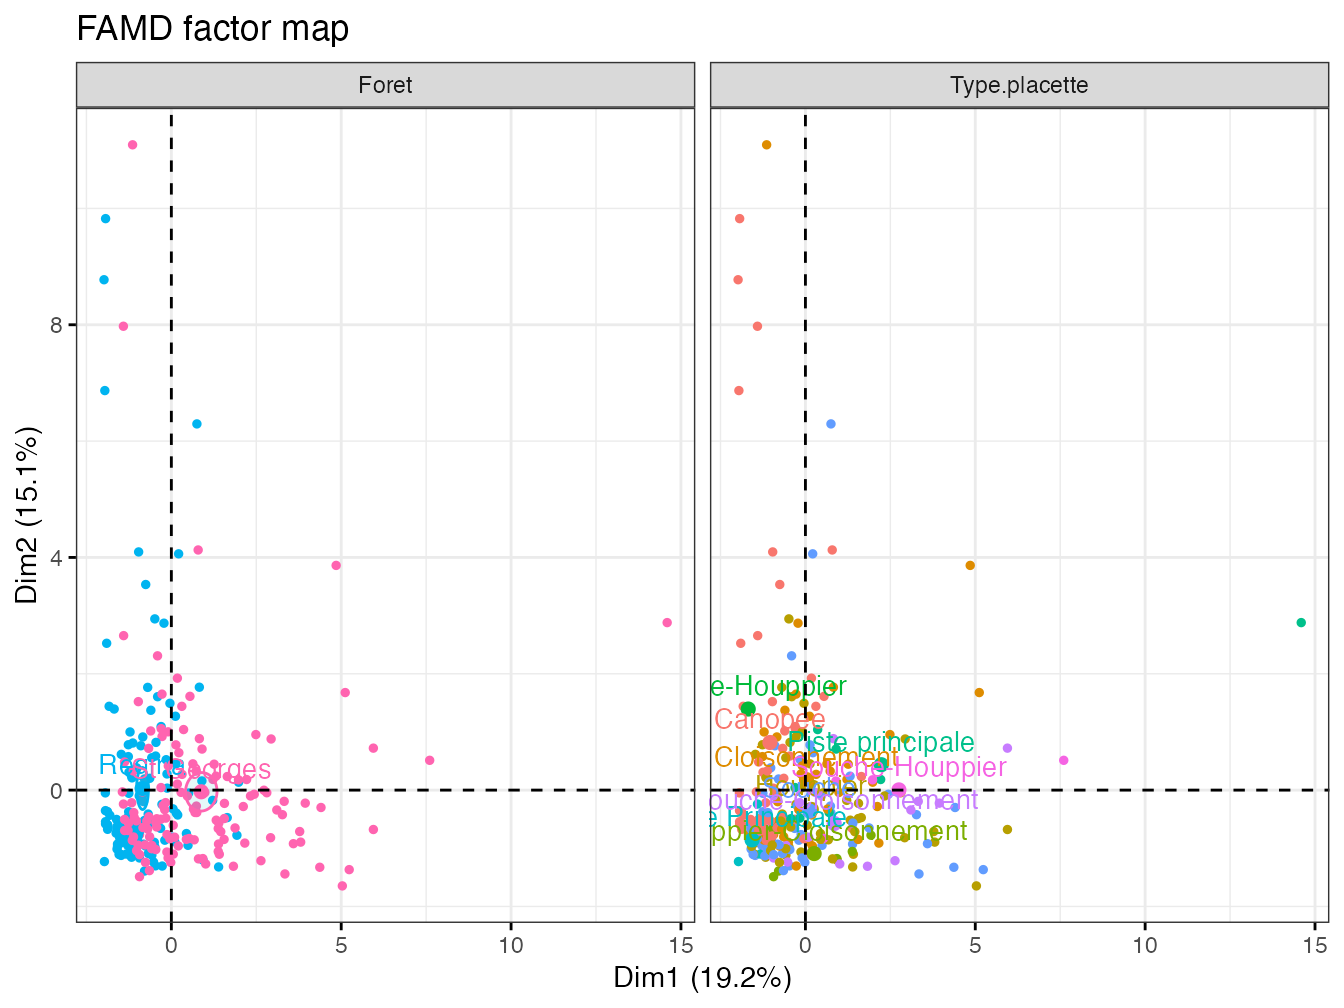
\includegraphics[width=0.8\linewidth]{MyBook_files/figure-latex/unnamed-chunk-9-5} \end{center}

\begin{Shaded}
\begin{Highlighting}[]
\CommentTok{\# individu extreme }
\end{Highlighting}
\end{Shaded}

\normalsize


% Bibliography
%%%%%%%%%%%%%%%%%%%%%%%%%%%%%%%%%%%%%%%%%%%%%%%%%%%%%%%%%%

\backmatter
\SmallMargins

\printbibliography
\onecolumn


% Tables (of tables, of figures)
%%%%%%%%%%%%%%%%%%%%%%%%%%%%%%%%%%%%%%%%%%%%%%%%%%%%%%%%%%


\cleardoublepage
\LargeMargins
\listoffigures


% After-body (LaTeX code inclusion)
%%%%%%%%%%%%%%%%%%%%%%%%%%%%%%%%%%%%%%%%%%%%%%%%%%%%%%%%%%




% Back cover
%%%%%%%%%%%%%%%%%%%%%%%%%%%%%%%%%%%%%%%%%%%%%%%%%%%%%%%%%%%

% Even page, small margins, no running head, no page number.
\evenpage
\SmallMargins
\thispagestyle{empty}

\begin{normalsize}

\begin{description}

\selectlanguage{english}
\item[Abstract]
English abstract, on the last page.

This is a bookdown template based on LaTeX memoir class.
\item[Keywords]
Keyword in English, As a list.
~\\

\end{description}

\end{normalsize}

\vspace*{\fill}
\centering\includegraphics[width=.3\textwidth]{images/logo}

\end{document}
